There does not exist among the literature a clearly defined comprehensive set of standard test scenarios as pointed out by \cite{MTT-Taxonomy}, which also notes that two types of scenarios of particular importance include crossing trajectories and parallel trajectories. With this in mind, we choose to generate scenarios of both trajectory types using a simple methodology that will be outlined in the following section. Furthermore, we evaluate our algorithms on two separate experiments, one with detection ambiguity and one without, with the first first outlined here in this section and the second outlined in the next. 

Both experiments and all steps including the scenario generation process, heuristic, and MIO were implemented in the development software \textit{julia} 0.4.3 \cite{julia} using the optimization package \textit{JuMP} \cite{JuMP}. The optimization software Gurobi 6.5.0 \cite{gurobi} was used to solve the MIOs, and the optimization processes was restricted to the use of a single core. Each simulation was run on a single compute node of the unclassified TX-Green cluster located at Lincoln Laboratories. The cluster utilizes DL165 G7 compute nodes, consisting of 2.2 GHz compute cores, with 8 GB of RAM each, for a total peak performance of 77.1 TFLOPS \cite{LLGrid}. 

\subsection{Scenarios without Detection Ambiguity}
In order to evaluate scalability of our algorithms we test our methods across a range of scenarios with varying numbers of targets and scans. In particular we consider: $ P \in \{4,6,8,10\}$ and $T \in \{4,6,8,10\}$ seconds. Scans are collected at a rate of 1 Hz. The cartesian product of $P$ and $T$ creates 16 unique scenario sizes. We generate 10 unique crossing scenarios and 10 unique parallel scenarios of each size. To generate trajectories, a grid size is first selected and then starting and stopping points are randomly selected within this grid. For crossing trajectories, the starting and stopping points have no restrictions, while for parallel trajectories the starting and stopping points are restricted to fall within subsets of the grid and these subsets are not allowed to overlap, resulting in trajectories that fall within close proximity to one another but do not overlap. For our experiments, a grid size of $[-10,10]$ was used. For each scenario, we randomly generate 10 realizations of data by first perturbing each true position measurement by an error $\epsilon \thicksim \mathcal{N}(0,\sigma)$ with $\sigma \in \{0.1,0.5,1.0,2.0,3.5,5.0\}$, where $\sigma$ represents the noise parameter. The problem data is then generated by adding the detection error to the true position:
\begin{align*}
	x_{it} = \alpha^{\text{true}}_{i} + \beta^{\text{true}}_{i}t+\epsilon.
\end{align*}

Scans $\mathcal{X}_{t}$ are simulated by randomizing the order of $x_{it}$ for each \textit{t}. Each unique $\boldsymbol{\mathcal{X}}$ generated is referred to as a \textit{simulation}. For each such simulation, we run the heuristic with a range of starting points $N \in \{100\ \ 1,000\ \ 10,000\}$, and use each of these solutions as a warm start for the MIO. The optimization process is set to terminate after 3T seconds, with solutions collected at intervals of $\{1,T,2T,3T\}$ seconds.

We begin the analysis of the methodologies by discussing the relationship between $\rho$ and $\sigma$ and discuss how this relationship benefits both scenario generation and complexity measuring by allowing each to occur in their own natural domain. Then we frame the performance of the basic heuristic before discussing the performance of the basic MIO model in both the data association and trajectory estimation spheres.

\subsubsection{Scenario Generation}
Figure~\ref{fig:Sigma_vs_Rho} shows the relationship between $\sigma$ and $\rho$ for our scenario generation methods. The plot is broken down by scenario type between crossing and parallel trajectories. 

\begin{figure}[ht]
  \centering
  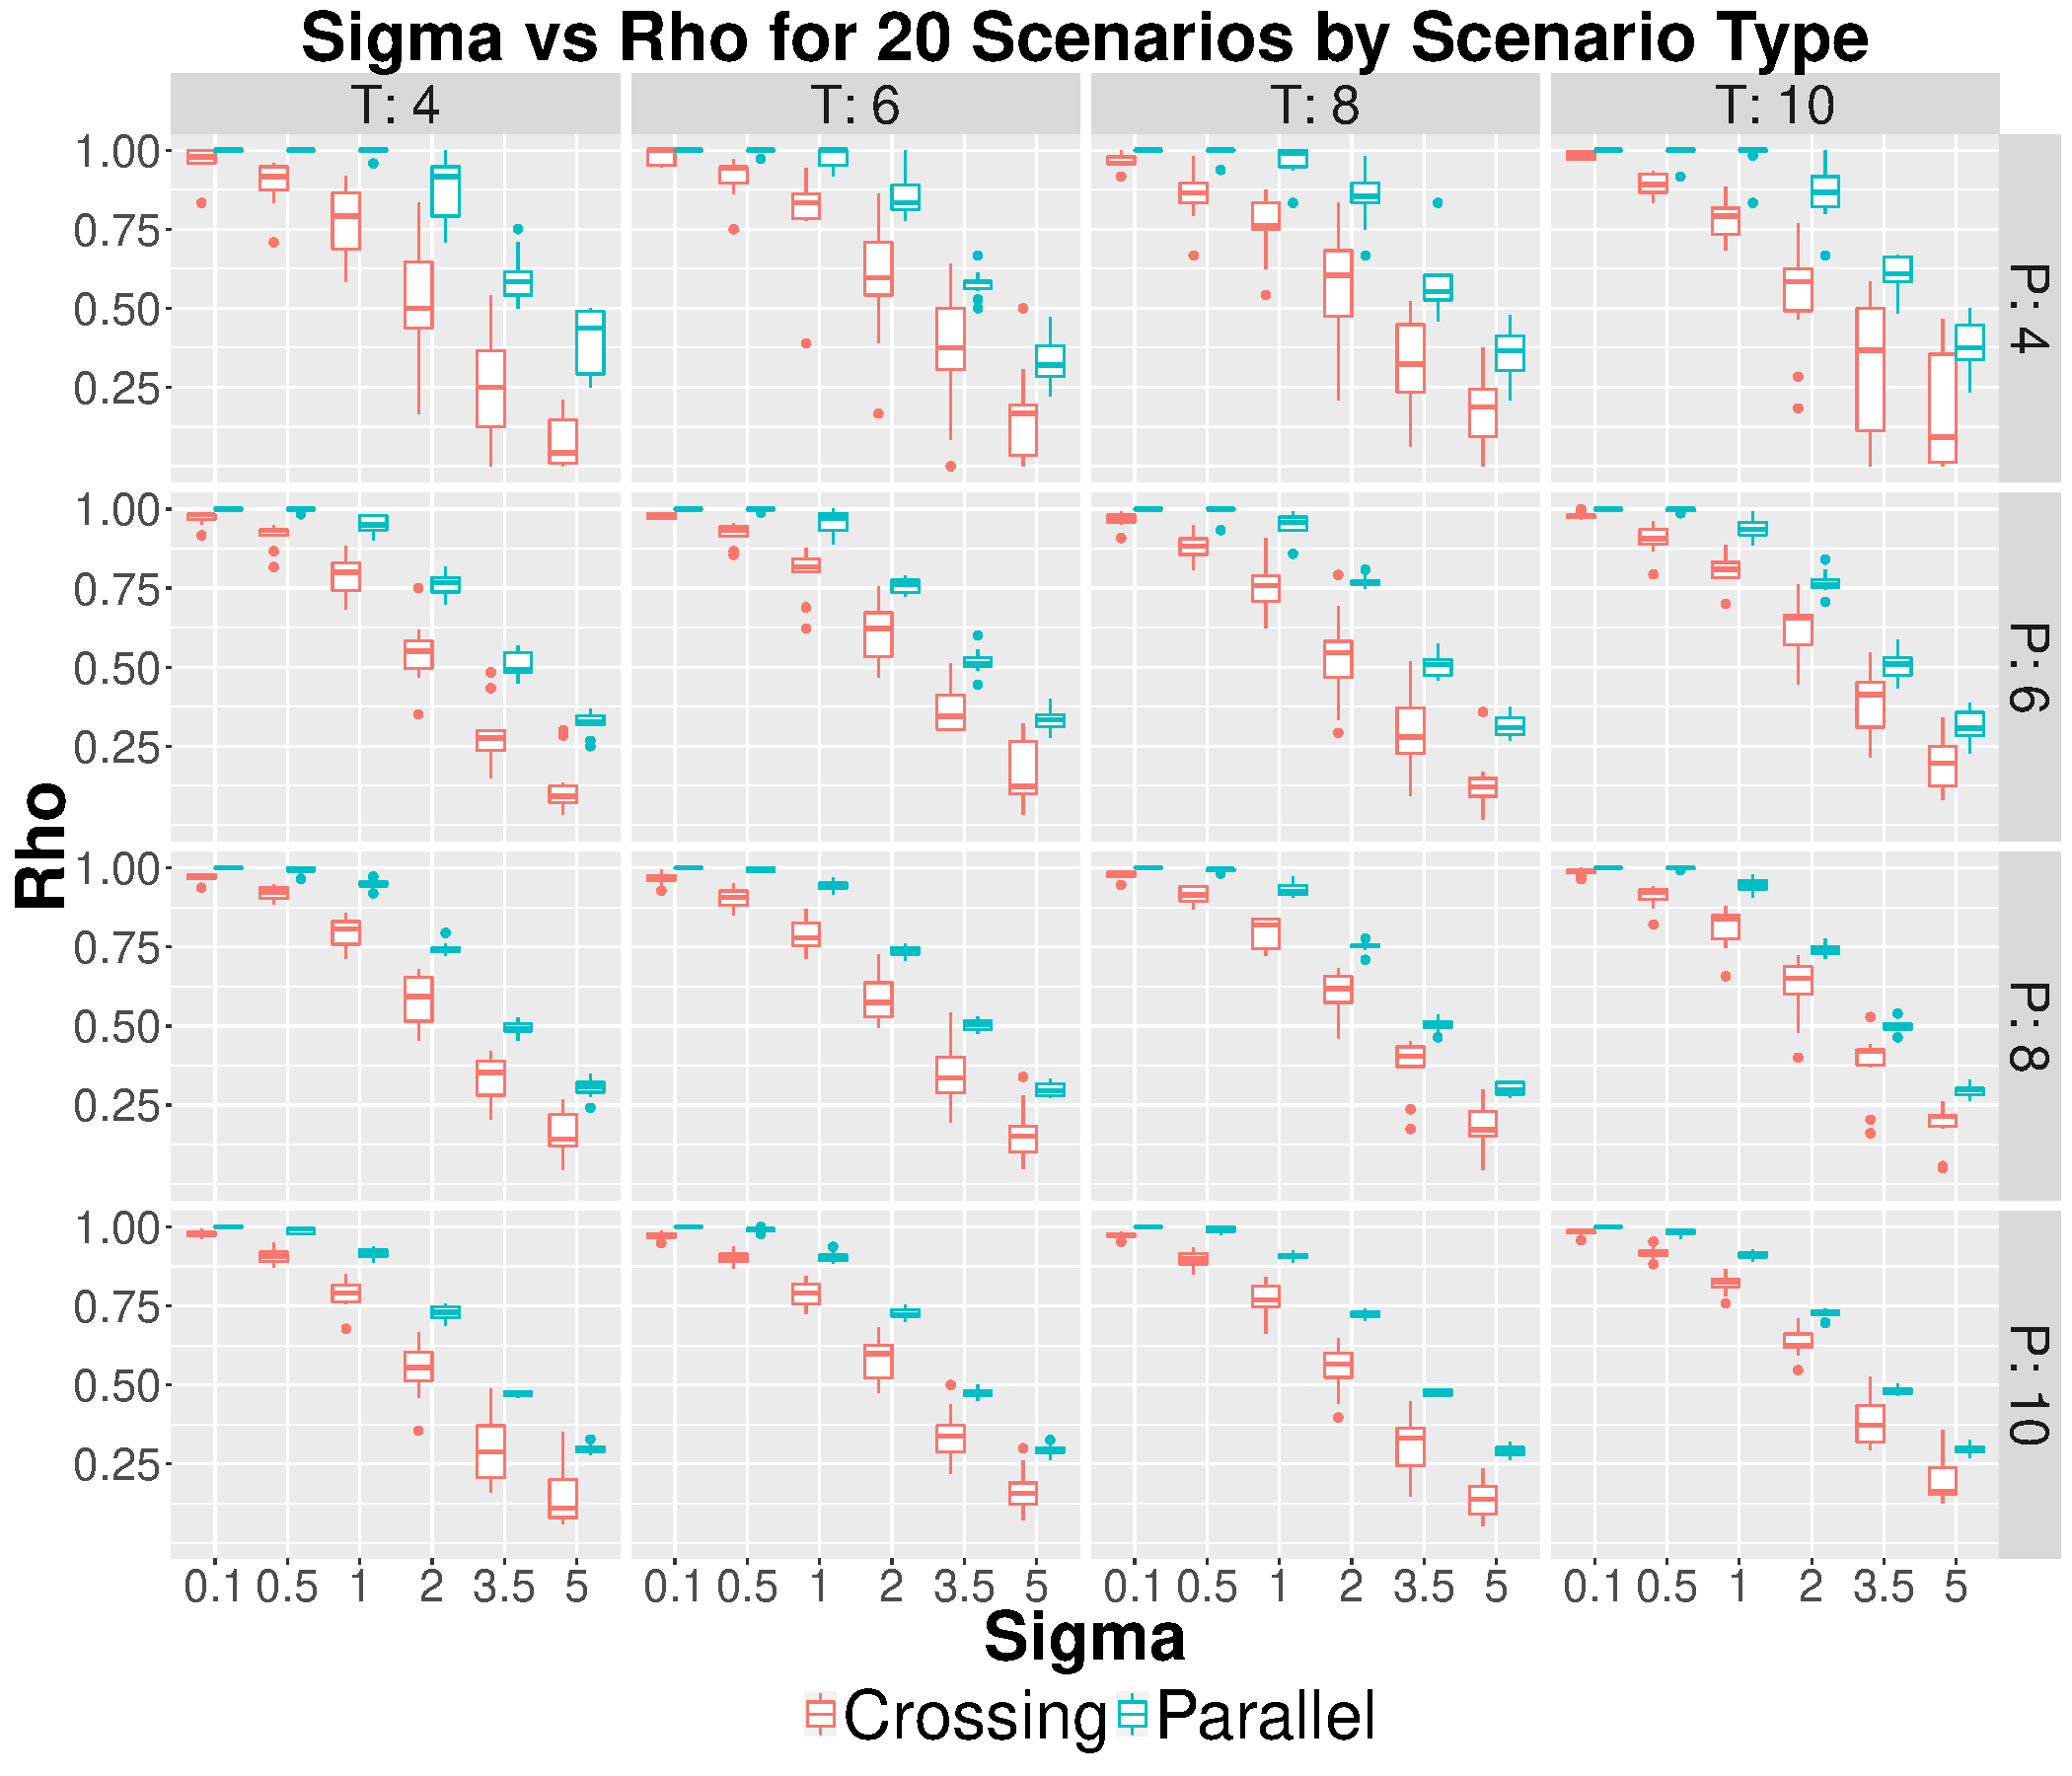
\includegraphics[width=\columnwidth]{../Figures//Sigma_vs_Rho}
    \caption{Relationship between $\sigma$ and $\rho$ summarized by scenario type for all 20 generated scenarios in this experiment.}
    \label{fig:Sigma_vs_Rho}
\end{figure}

It can be seen that the parallel method of scenario generation on the average creates easier scenarios for the data association problem, as measured by $\rho$,. This result supports the hypothesis that crossing scenarios would be more likely to exhibit detections within close proximity, and consequently result in more difficult scenarios as it pertains to the data association problem. 

In addition, we see from this plot that a relatively small range of six values of $\sigma$ corresponds to the full range of $\rho$ from 0 to 1, meaning that we can quantify data association performance across a more continuous range. This means that $\sigma$ can be used in its natural domain of the data generation process, and $\rho$ can be back calculated as a measurement of difficulty for the data association problem. As a result, we gain a highly interpretable performance metric for the data association problem without sacrificing the ability to generate scenarios in their natural domain. 

\subsubsection{Basic Heuristic}
We begin our discussion of the heuristic with an examination of the run times from the experiment. Table~\ref{tab:Basic_heuristic_times} summarizes the minimum, mean, and maximum run times of the heuristic from this experiment for a single starting point, arranged by the number of targets ($P$) and number of scans ($T$). Times are shown in milliseconds. 

\begin{table}[ht]
\centering
\begin{tabular}{cc|ccc}
  \hline
   & & \multicolumn{3}{c}{Heuristic Run Times } \\
   & & \multicolumn{3}{c}{(in milliseconds)}\\
   P & T & Min & Mean & Max \\ 
  \hline
  \hline
   4 & 4 & 0.07 & 0.10 & 0.18 \\ 
   4 & 6 & 0.18 & 0.24 & 0.38 \\ 
   4 & 8 & 0.34 & 0.45 & 0.62 \\ 
   4 & 10 & 0.58 & 0.76 & 1.02 \\ 
   6 & 4 & 0.11 & 0.15 & 0.25 \\ 
   6 & 6 & 0.31 & 0.39 & 0.58 \\ 
   6 & 8 & 0.64 & 0.81 & 1.05 \\ 
   6 & 10 & 1.24 & 1.56 & 2.02 \\ 
   8 & 4 & 0.14 & 0.19 & 0.30 \\ 
   8 & 6 & 0.46 & 0.57 & 0.86 \\ 
   8 & 8 & 0.95 & 1.24 & 1.58 \\ 
   8 & 10 & 2.07 & 2.53 & 3.37 \\ 
   10 & 4 & 0.19 & 0.25 & 0.41 \\ 
   10 & 6 & 0.63 & 0.80 & 1.03 \\ 
   10 & 8 & 1.44 & 1.84 & 2.44 \\ 
   10 & 10 & 2.96 & 3.73 & 4.56 \\ 
   \hline
\end{tabular}
\caption{Heuristic run times (in milliseconds) for a single starting point.}
\label{tab:Basic_heuristic_times}
\end{table}

Notice that the number of scans has a much greater effect on run times than the number of targets. Whereas the average run time roughly doubles with each increase of 2 scans, the average run time increases as little as 27\% but no more than 50\% for each increase of 2 targets. Therefore, the heuristic scales much more efficiently with $P$ than $T$. Although this may initially seem like a cause for concern, this is actually a desirable trait because it suggests that the heuristic is likely a good candidate for use in a sliding window algorithm. Rather than solve all scans in a single batch at once, a sliding window algorithm solves a subset of scans, or a smaller window, and advances through all scans sequentially.  As the window progresses forward through the scans, "soft" decisions are made meaning that the heuristic would begin with the decisions from the previous solution. As scans pass beyond the horizon and out of the sliding window, the decisions become fixed and we refer to them as "hard" decisions. This process continues until all scans have been processed. The run times of a sliding window variant of the heuristic would not exhibit the curse of dimensionality in $T$ since the number of scans remains constant. Additionally, the heuristic is likely to produce higher quality solutions as a result of these "soft" decisions of previous steps since it is starting from a solution which is likely to be better than a completely random solution. 


Furthermore, the heuristic is extremely parallelizable. This means that we can run different sets of starting points for the heuristic on several computers, allowing either a reduction in total run time for a fixed number of starting points or an increase in the number of starting points for a fixed run time. For example, the average run time for a single starting point of a scenario of six targets and six scans is about 0.4 milliseconds. If we desire to evaluate 50,000 heuristic starting points, we would require about 20 seconds of run time if run in sequence. However, the same number of starting points parallelized onto 100 processors would reduce the total run time to approximately 0.2 seconds. Thus, the run time of the heuristic can be reduced to meet the efficiency needs of the system subject only to the limitation of available processors. 

We continue our evaluation of the basic heuristic by analyzing the performance of its solution on the MIO objective. This gives insight into whether or not the use of RSS as a proxy for the MIO objective is effective. To evaluate effectiveness on these terms, we compute the corresponding MIO objective value of the heuristic solution and normalize it against the MIO objective value of the \textit{ideal} solution, which refers to the solution in which the data association problem is exactly correct (all detection assignments are exactly known). The resulting normalized value represents the MIO objective value as a factor of the ideal solution's MIO objective value. This metric is plotted against $\sigma$ and summarized in Figure~\ref{fig:Basic_Heuristic_Objective}. 

\begin{figure}[ht]
  \centering
  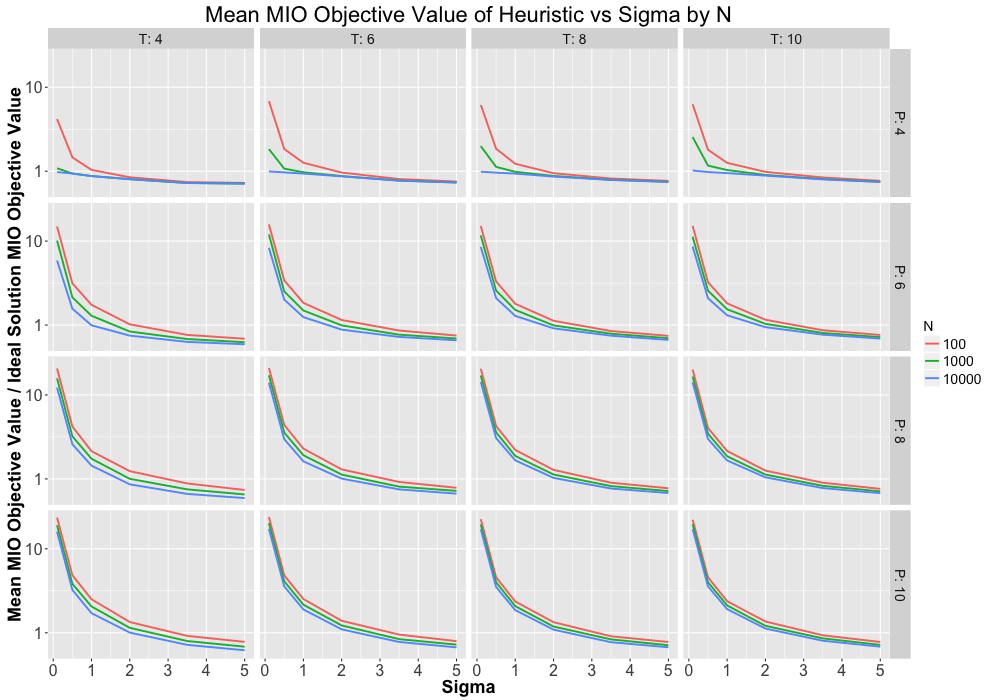
\includegraphics[width=\columnwidth]{../Figures/Basic_Heuristic_Objective}
  \caption{Heuristic performance as a factor of the ideal solution's MIO objective value.}
  \label{fig:Basic_Heuristic_Objective}
\end{figure}

We see that increasing the number of starting points improves the quality of the heuristic solution as compared to the ideal solution's MIO objective value, especially when the number of targets is small. However, this effect is diminished as the number of targets increases. In addition, we see that for larger numbers of targets, even the largest number of starting points does not achieve near ideal performance, suggesting the need for a much larger number of starting points. This is not considered to be a problem, however, due to the advantages of parallelization discussed previously and also due to the power of optimization, which we will see later. 

We also see that for larger values of $\sigma$ the heuristic actually outperforms the ideal solution's MIO objective value. Remember that the ideal solution is simply ideal in the sphere of data association, while the MIO objective intends to score both the data association and trajectory estimation simultaneously. Therefore, we draw the conclusion that achieving perfect data association for large values of sigma does not necessarily correspond to the best solution to the trajectory estimation problem. In other words, as $\sigma$ increases it may be necessary to tradeoff correct data associations in order to improve the trajectory estimation. We believe the results of the heuristic could be explained by this effect.

Next, we evaluate the performance of the basic heuristic on the data association problem as a function of the number of starting points. To this end, we relationship between accuracy and $N$. Figure~\ref{fig:Basic_Heuristic_Accuracy} plots the mean accuracy of each of the three starting points from this experiment against $\rho$. 

\begin{figure}[ht]
  \centering
  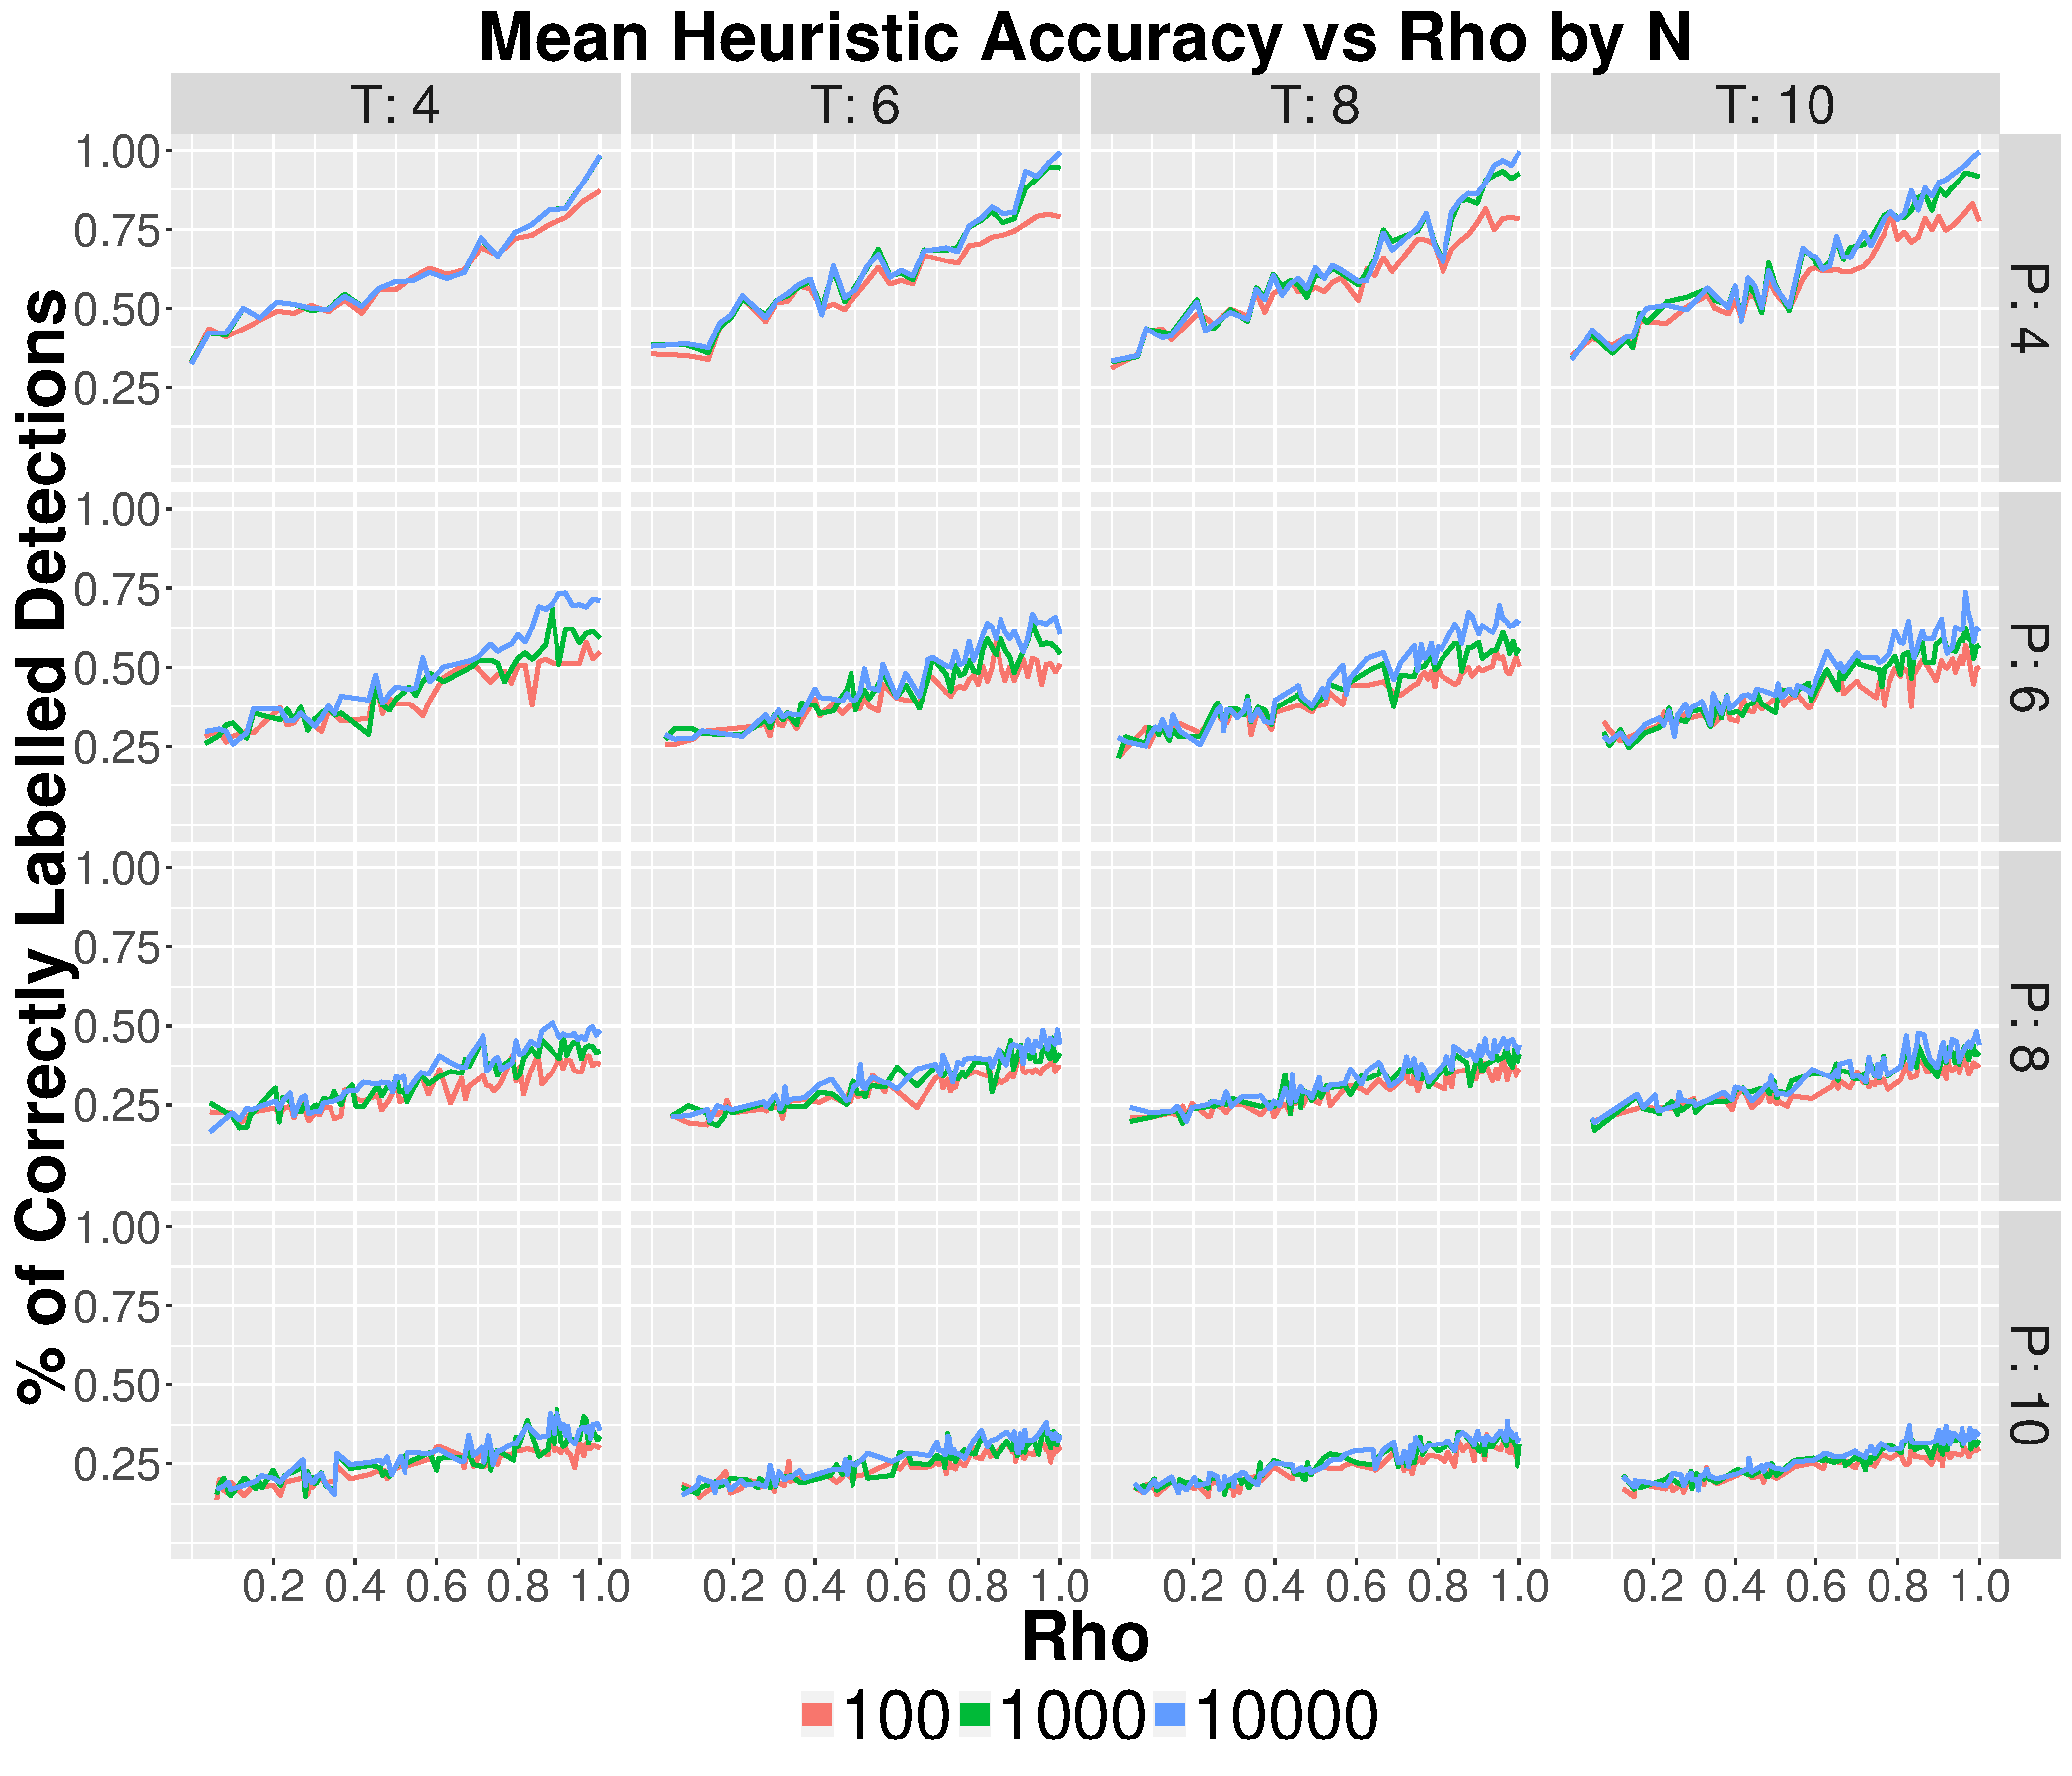
\includegraphics[width=\columnwidth]{../Figures/Basic_Heuristic_Accuracy}
  \caption{Accuracy of basic heuristic by number of heuristic starting points.}
  \label{fig:Basic_Heuristic_Accuracy}
\end{figure}

First of all, we see that the heuristic finds good solutions to the data association problem, especially for scenarios with fewer targets, but performance degrades as the number of targets increases which is expected. Again it is seen that increasing the number of starting points results in minor improvements, and this improvement is greatest for scenarios with fewer targets. We see a similar effect as $\rho$ increases. We conclude that even small values of $N$ produce moderately good solutions as measured by accuracy.

Overall we conclude that there is not a significant difference in heuristic performance for the range of $N$ values that we explored. Therefore for simplification as we move forward in our analysis, we will restrict our discussions of the heuristic to $N=1,000$.

\subsubsection{Basic MIO}
Next, we transition our evaluation to focus on the MIO by first measuring its performance on the data association problem. Figure~\ref{fig:Basic_Accuracy_Summary} plots the mean accuracy of the MIO, initialized by the $N=1,000$ heuristic solutions, after 1,T, and 2T seconds against $\rho$. We have excluded the data for the MIO after 3T seconds for the sake of clarity as it showed little to no improvement over the MIO after 2T solution. For comparison, we have included the heuristic (for $N=1,000$ only) in addition to a randomized solution, one in which we randomly assigned detections to targets. Note that in this case, that the ideal solution, one in which the associations are exactly correct, achieves an accuracy of 1.0 in all cases so it is not shown explicitly.

\begin{figure}[ht]
  \centering  
  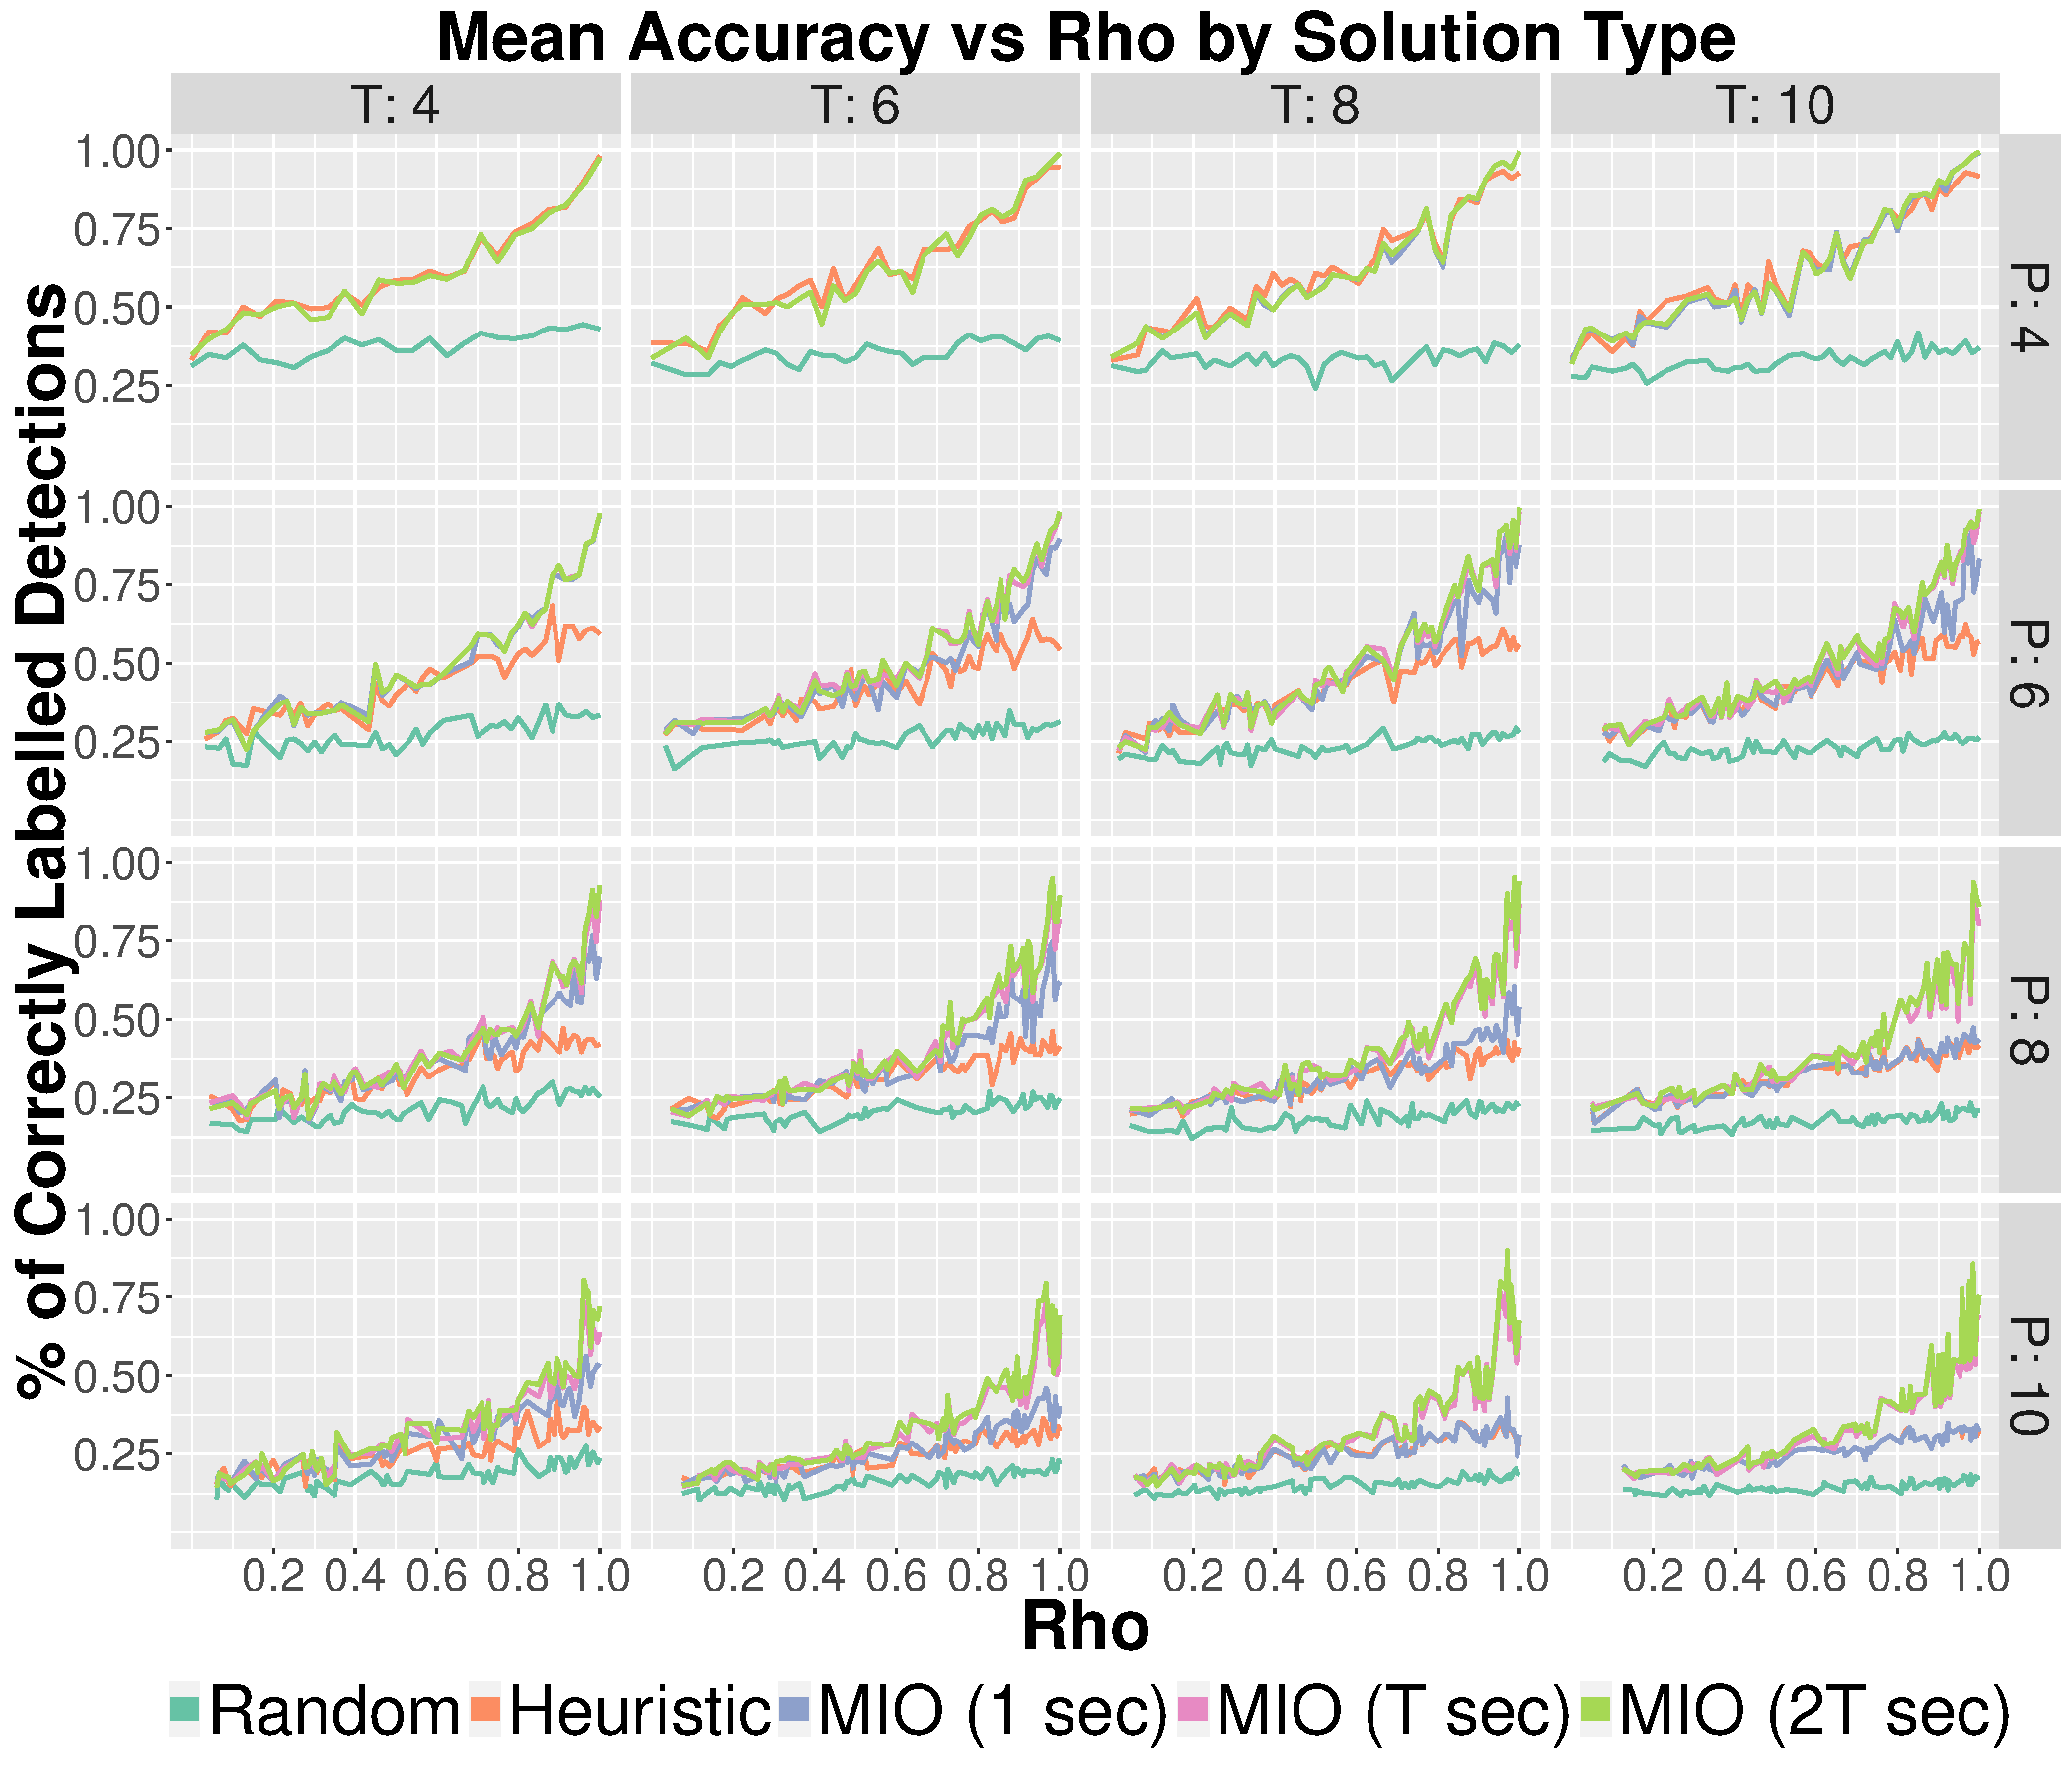
\includegraphics[width=\columnwidth]{../Figures/Basic_Accuracy_Summary}
  \caption{Accuracy of MIO compared against the heuristic and a randomized solution.}
  \label{fig:Basic_Accuracy_Summary}
\end{figure}

For scenarios with fewer numbers of targets, the MIO solutions were actually proven to be the optimal solution. Therefore, for smaller scenarios with few targets, we see that the heuristic achieves optimal and near optimal solutions. We also see that the easier the scenario, the more improvement the MIO has over the heuristic, while in more difficult scenarios the effect is diminished. Furthermore, it can be seen that in nearly all scenarios, the MIO achieves its best or near best solutions after $T$ or fewer seconds, suggesting the usefulness of the MIO as an online algorithm with a sliding window. 

As mentioned previously in regards to the heuristic, a sliding window algorithm would make decisions on a subset of scans, and these decisions will be fixed before accepting a new set of scans. In regards to the MIO, this would be implemented by adding constraints to restrict the values of $y_{itj}$ to match that of the subsetted solution. The fact that the MIO finds very good solutions in $T$ or fewer seconds means that a sliding window algorithm would be able to solve each subset in real time before advancing to the next subset of scans. Furthermore, the MIO would likely benefit from the fixed decisions of the preceding windows, since this is added knowledge that has not utilized by our approaches.

Next, we evaluate the performance of the basic heuristic and MIO through the lens of trajectory estimation. As discussed previously, we are interested in comparing $\delta$, our proxy for ground track error, against $\sigma$, our measure of difficulty for trajectory estimation, in order to analyze performance of in the sphere of estimation. Figure~\ref{Fig:Basic_Delta_Summary} plots $\sigma$ against $\delta$ for each of the solution types. In addition to the random solution shown on the previous plot, we also add a comparison to the ideal solution, as previously defined.
\begin{figure}[ht]
  \centering
  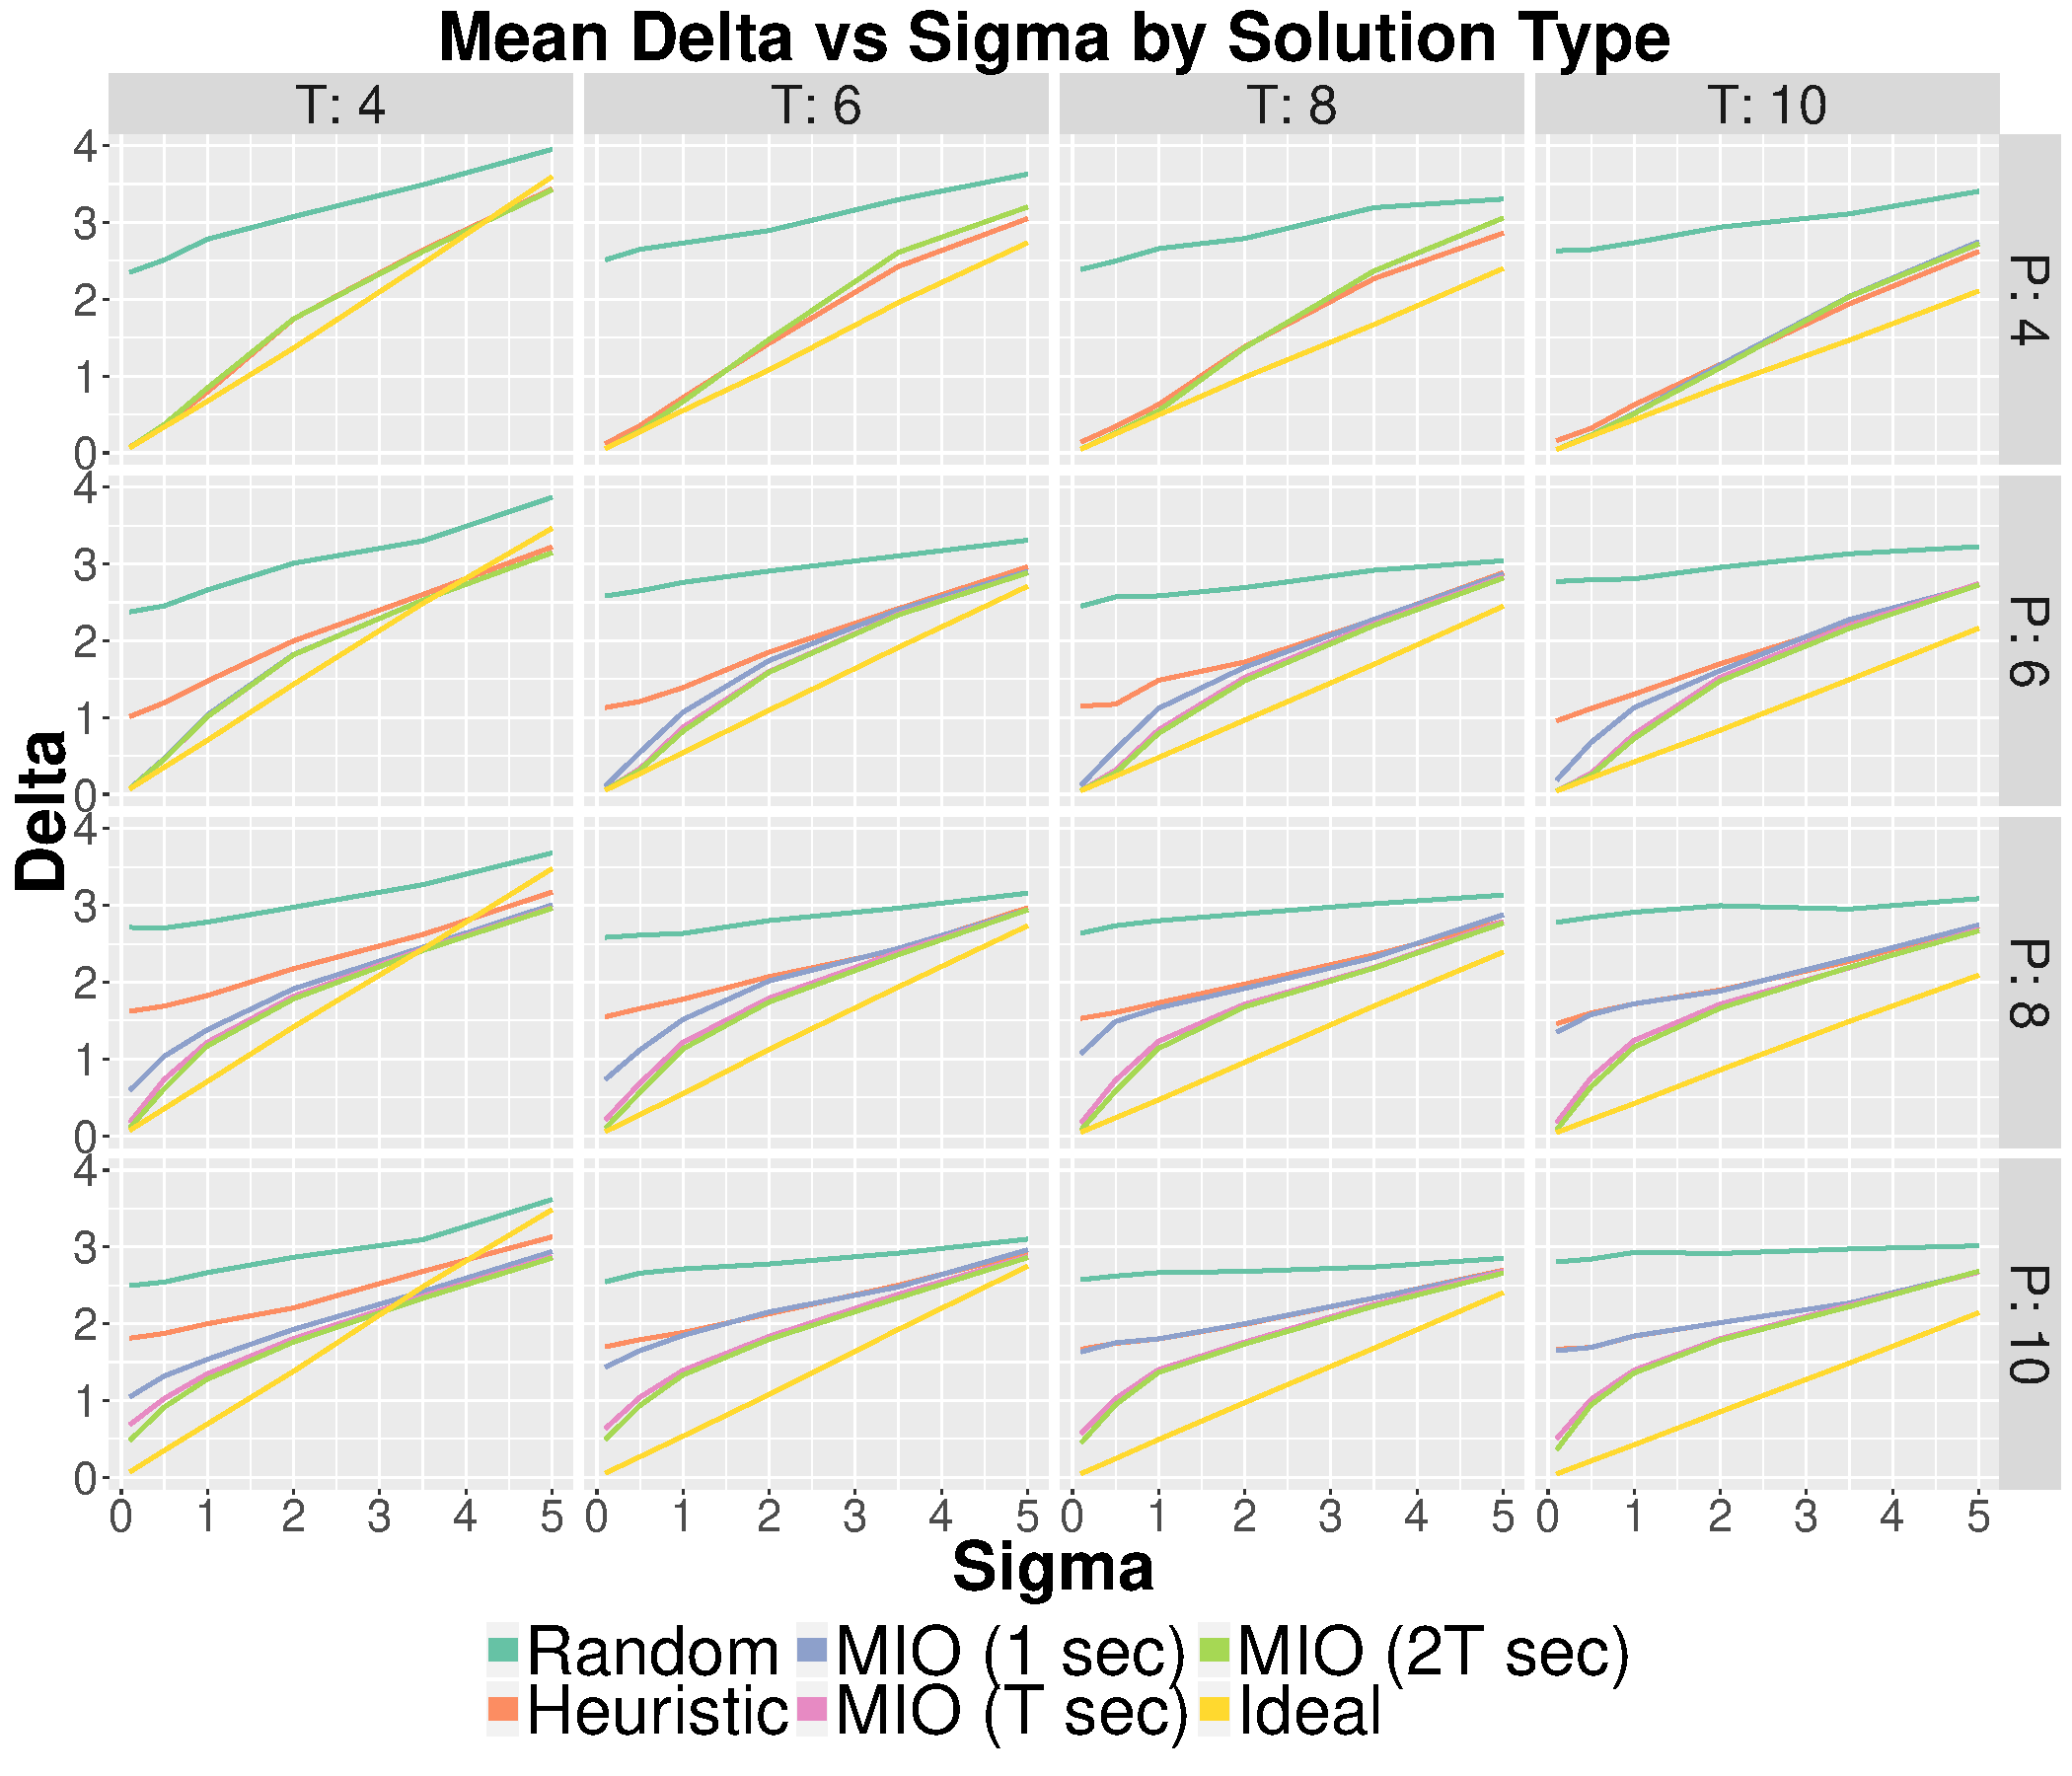
\includegraphics[width=\columnwidth]{../Figures/Basic_Delta_Summary}
  \caption{Trajectory estimation performance}
  \label{Fig:Basic_Delta_Summary}
\end{figure}

Remember that lower values of delta correspond to trajectory estimations that are closer to that of the true ground track. We see that the performance of the heuristic converges to that of the MIO for scenarios with few targets, as well as for large values of $\sigma$. Additionally, we see that as the number of targets increases we begin to see stronger improvements by the MIO over the heuristic. Interestingly, we see that for the scenarios with the largest number of targets and scans, the MIO after one second is not much better than the heuristic. While the MIO after T seconds provides significant improvement over that of the heuristic and MIO after 1 second, there is little further improvement in running the MIO for 2T seconds. 

Again, we see that in scenarios with only for scans ($T=4$) we see that for larger values of $\sigma$ the heuristic and/or MIO sometimes outperforms the ideal. This is likely a result of limited data and increases uncertainty under high noise. As the number of scans approaches infinity, the ideal solution, or perfect data associations, leads to trajectory estimates that are closer and closer to the true ground track. Put differently. as more and more data is known, it becomes easier to estimate the trajectories even in the event of large noise, and so the trajectory estimates that result from the ideal solution converges to the true ground track. 

In summary, we have shown that in the case of no detection ambiguity, our methods are scalable and provide high quality solutions in milliseconds. The heuristic scales especially well in respect to increases in the number of targets. The scalability in regards to increases in the number of scans can be mitigated through the aid of parallelization. The heuristic shows good  as warm starts for the MIO. The MIO achieves high quality solutions in 

\subsection{Scenarios with Detection Ambiguity}
Here we extend the discussion from the previous section to analyze the performance of our methods on scenarios with detection ambiguity. We first summarize our experimental methods before discussing performance of both the robust heuristic and the robust MIO in the spheres of both the data association and trajectory estimation problems.

This experiment serves as an extension of the basic one, in order to test the performance of our algorithms under detection ambiguity. We use the same scenarios generated from the basic experiment, but due to the additional difficulty inherent with detection ambiguity, we limit the range of signal noise to $\sigma \in \{0.1,0.5,1.0,2.0\}$, excluding choosing to exclude the extreme cases of signal noise. In addition, we simulate both missed detections and false alarms. A detection is removed with probability, $\gamma$, and we consider $\gamma \in \{0.2,0.15,0.1,0.05\}$. We do not allow empty scans. For each scan, we generate false alarms according to a poisson distribution with parameter, $\lambda$, and detection locations are then randomly selected uniformly within the state space. We consider $\lambda \in \{0.1,0.5,0.1,2.0\}$. The false alarms are then added to $\mathcal{X}_{t}$ and the detection order of $\mathcal{X}_{t}$ is again randomly shuffled as before. 

Once the data has been generated, we follow the same sequence as before in the basic experiment, running the heuristic first and then feeding the solution into the MIO as a warm start. Note that the heuristic is given 1,000 starting points only, as concluded from the results of the basic experiment. Once again, the optimization process was set to terminate after 3T seconds, with solutions collected at intervals of $\{1,T,2T,3T\}$ seconds. Prior to the running of this experiment, we performed a mini experiment and used the results to tune the penalties $\theta$ and $\phi$. A summary of the exact penalties used along with an explanation of the insight behind them, can be found in Appendix~\ref{\myabrv Penalty_Appendix}. 

We will now evaluate the performance of the robust heuristic and MIO. We begin with a discussion on the run times of the robust heuristic, following the number of targets estimation, accuracy and trajectory estimation.

\subsubsection{Robust Heuristic Run Times} Table~\ref{tab:Robust_heuristic_times} summarizes the minimum, mean, and maximum run times of the heuristic from Experiment 2 for a single starting point, arranged by the number of estimate targets ($P_{estimated}$) and number of scans ($T$). Times are shown in milliseconds. 

\begin{table}[ht]
\centering
\begin{tabular}{cc|ccc}
  \hline
   & & \multicolumn{3}{c}{Heuristic Run Times } \\
   & & \multicolumn{3}{c}{(in milliseconds)}\\
   $ P_{\text{estimated}}$ & T & Min & Mean & Max \\ 
  \hline
  \hline
  2 & 4 & 0.15 & 0.23 & 0.41 \\ 
  2 & 6 & 0.42 & 0.56 & 0.93 \\ 
  2 & 8 & 0.77 & 1.04 & 2.24 \\ 
  2 & 10 & 1.27 & 1.73 & 20.23 \\ 
  4 & 4 & 0.15 & 0.34 & 1.04 \\ 
  4 & 6 & 0.50 & 0.94 & 2.69 \\ 
  4 & 8 & 1.09 & 1.88 & 3.87 \\ 
  4 & 10 & 2.12 & 3.25 & 13.51 \\ 
  6 & 4 & 0.14 & 0.42 & 0.96 \\ 
  6 & 6 & 0.57 & 1.29 & 4.45 \\ 
  6 & 8 & 1.33 & 2.66 & 75.28 \\ 
  6 & 10 & 2.53 & 4.61 & 18.69 \\ 
  8 & 4 & 0.16 & 0.50 & 1.10 \\ 
  8 & 6 & 0.60 & 1.59 & 3.46 \\ 
  8 & 8 & 1.38 & 3.37 & 6.87 \\ 
  8 & 10 & 2.63 & 5.84 & 12.40 \\ 
  10 & 4 & 0.18 & 0.55 & 1.10 \\ 
  10 & 6 & 0.72 & 1.82 & 3.98 \\ 
  10 & 8 & 1.53 & 3.96 & 8.18 \\ 
  10 & 10 & 3.42 & 6.93 & 13.93 \\ 
  12 & 4 & 0.16 & 0.56 & 0.99 \\ 
  12 & 6 & 0.99 & 1.95 & 3.96 \\ 
  12 & 8 & 1.74 & 4.33 & 8.69 \\ 
  12 & 10 & 3.40 & 7.71 & 15.10 \\ 
   \hline
\end{tabular}
\caption{Robust heuristic run times (in milliseconds) for a single starting point.}
\label{tab:Robust_heuristic_times}
\end{table}

Comparing Table~\ref{tab:Basic_heuristic_times} and Table~\ref{tab:Robust_heuristic_times} we see that the run times for an estimated number of targets in the robust heuristic range from roughly double to three and four times that of a comparable number of targets in the basic heuristic. Due to the increase in combinatorial solutions in the robust heuristic over the basic heuristic, this was an expected result. The robust heuristic, however, can be parallelized in the same many as the basic heuristic, meaning that the robust heuristic can actually recover the speed of the basic heuristic with the introduction of additional processors. More importantly, we see that the robust heuristic scales very efficiently with $P_{\text{estimated}}$, and this the scaling actually improves as the number of estimated targets and scans increases. Increasing from two to six estimated targets for four scans roughly triples the run time, while increasing from eight to twelve estimated targets for four scans increases the run time by only 12\%. This is a great result because it means that a relatively wide range of estimated targets can be parallelized without fear of one subset requiring a substantially longer run time than another. 

Although the robust heuristic scales well with the number of estimated targets, it is more sensitive to increases in the number of scans. However, this effect is no worse than what we saw for the basic heuristic. It appears that on average increasing the number of scans by 2 results in a doubling of the run time for a fixed number of estimated targets. We conclude that these results again support the use of the robust heuristic in an online algorithm with a sliding window, as discussed in the previous section.
 
\subsubsection{Evaluating the Number of Targets}
Next, we continue our analysis of the robust approaches by quantifying the algorithms' ability to estimate the correct number of targets. This is perhaps the most important goal of a MTT algorithm and so we begin our analysis here. To this end, we define
\begin{align}
	P_{\text{diff}} = P_{\text{true}} - P_{\text{est}}
\end{align}

where $P_{\text{estimated}}$ is the number of estimated targets and $ P_{\text{true}}$ is the number of true targets, and we plot the distribution of $P_{\text{estimated}}$. Figure~\ref{fig:Robust_4_8_Histogram} shows the distribution of $P_{\text{difference}}$ for scenarios with four targets and eight scans, and for comparison, Figure~\ref{fig:Robust_8_8_Histogram} plots the same result for scenarios of eight targets and eight time scans. 
\begin{figure}[ht]
  \centering
  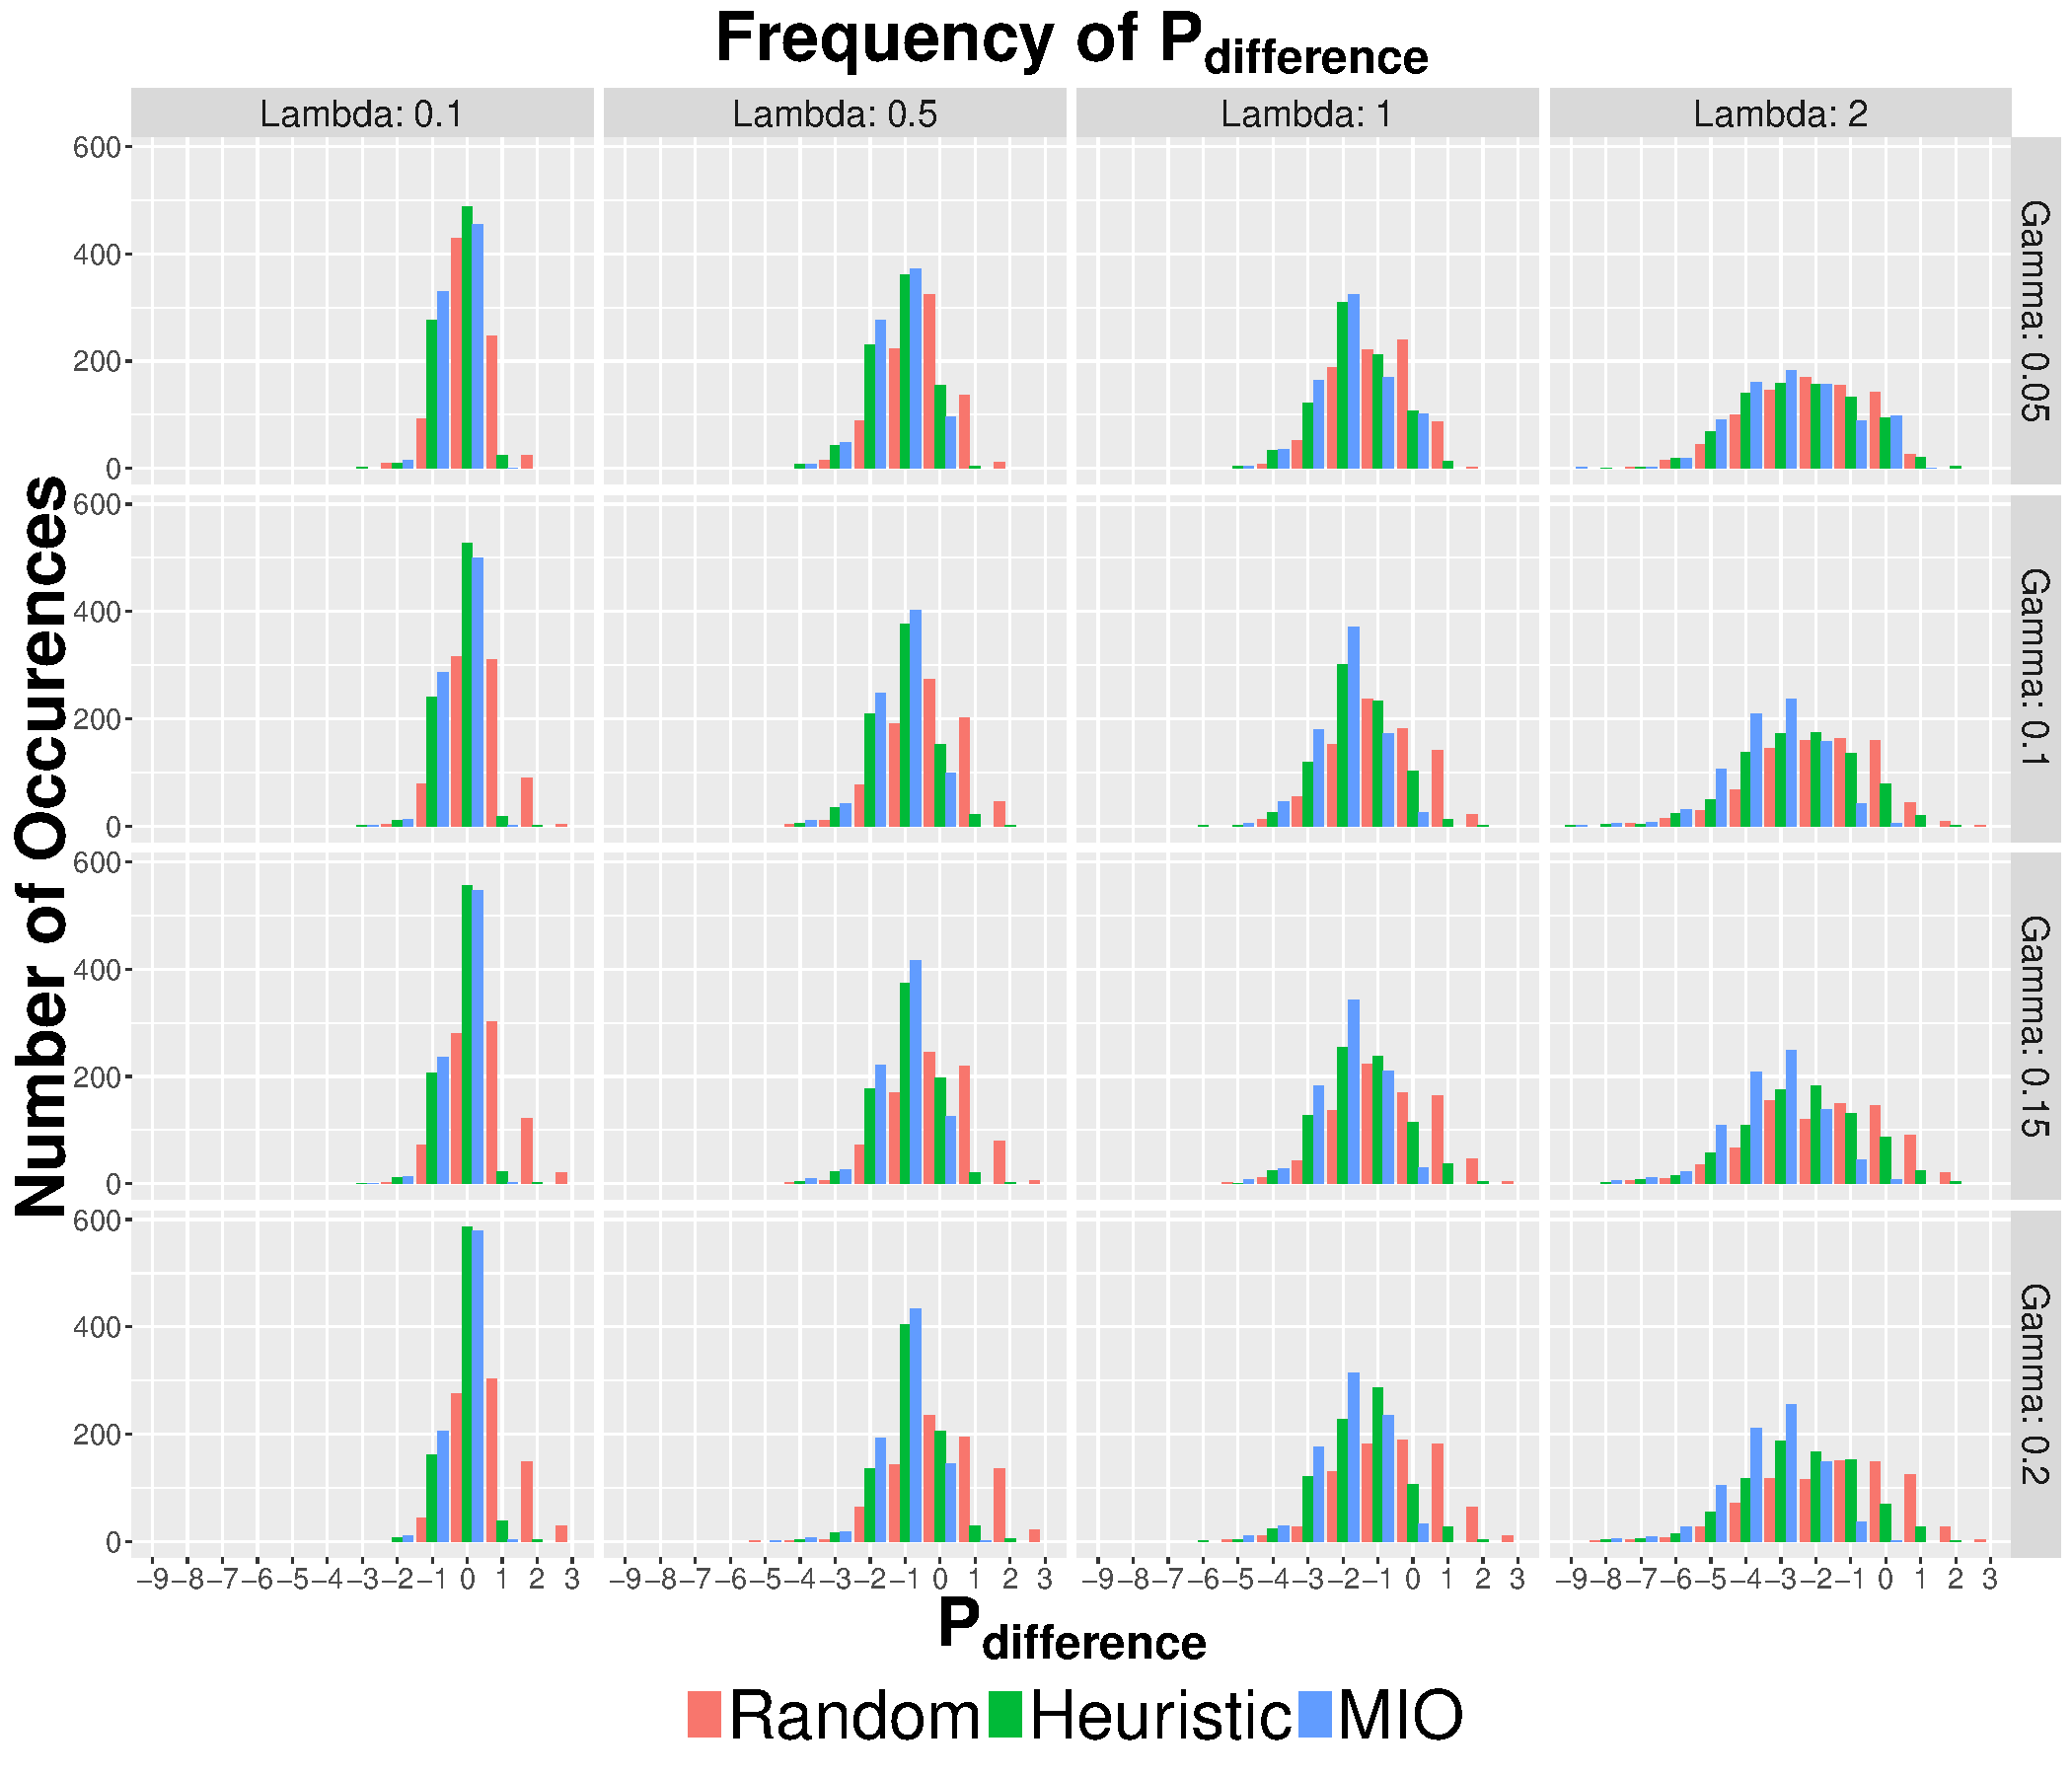
\includegraphics[width=\columnwidth]{../Figures/4_8_Histogram}
  \caption{Distribution of the difference in true and estimated number of targets for scenarios with 4 targets and 8 scans, arranged by $\gamma$ and $\lambda$.}
  \label{fig:Robust_4_8_Histogram}
\end{figure}

\begin{figure}[ht]
  \centering
  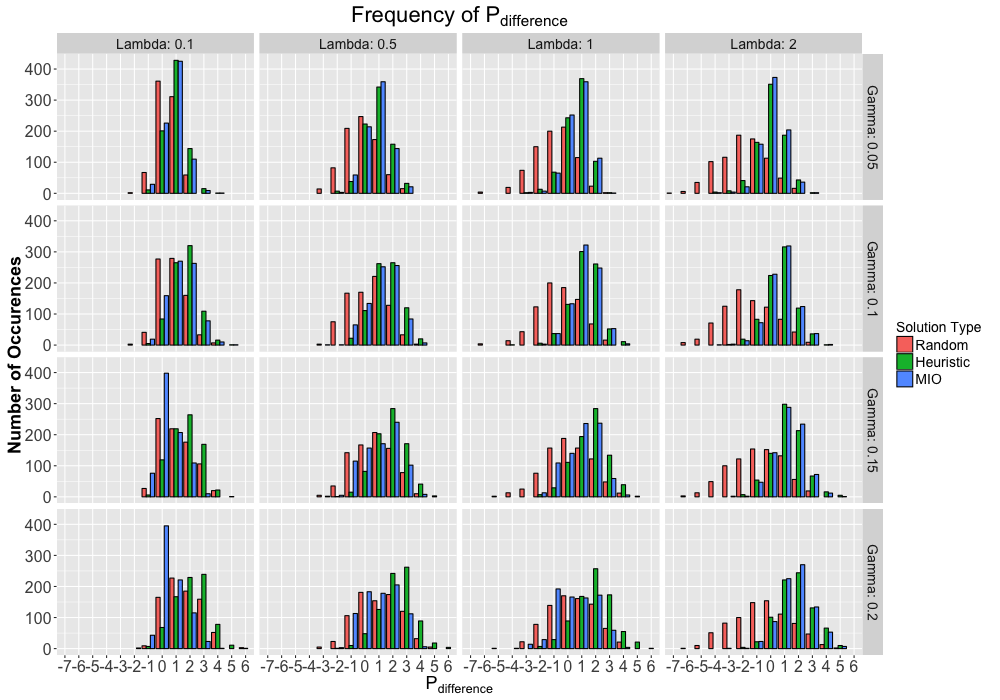
\includegraphics[width=\columnwidth]{../Figures/8_8_Histogram}
  \caption{Distribution of the difference in true and estimated number of targets for scenarios with 8 targets and 8 scans, arranged by $\gamma$ and $\lambda$.}
  \label{fig:Robust_8_8_Histogram}
\end{figure}

Note that the algorithms have correctly estimated the number of targets when $P_{\text{difference}} = 0$. When $P_{\text{difference}} < 0$, we have overestimated the number of targets, and when $P_{\text{difference}} > 0$, we have underestimated the number of targets. We see that both the robust heuristic and the robust MIO estimate the number of targets correctly a high proportion of the time in the scenario with four targets, particularly for smaller values of $\lambda$. As $\lambda$ increases, though, both algorithms tend to underestimate. The same trend persists in the larger scenario. This suggests that either 1) the false alarm penalty needs further tuning and likely was not set high enough in the experiment or 2) the missed detection penalty set too high. In the case where $\theta$ is set too low, the algorithms would prefer to classify detections as false alarms rather than create additional trajectories for the detections. In the case of $\phi$ set too high, the algorithms would opt out of creating additional trajectories in order to decrease the need to fill smaller scans with missed detections. Furthermore, because the effect of underestimation is more prominent in the scenario with more targets, we conclude that both penalties should probably take into account the number of targets that it is currently estimating.

\subsubsection{Data Association}
Knowing that we tend to underestimate the number of targets with the given penalties, we move on in our analysis to measuring the accuracy of our robust approaches. Figures~\ref{fig:Robust_4_8_Accuracy} and~\ref{fig:Robust_8_8_Accuracy} plot the accuracy performance metric against the difficulty metric, $\rho$, for scenarios of four and eight targets, respectively. Both scenarios have eight scans and both Figures have been arranged by $\gamma$ and $\lambda$.
\begin{figure}[ht]
  \centering
  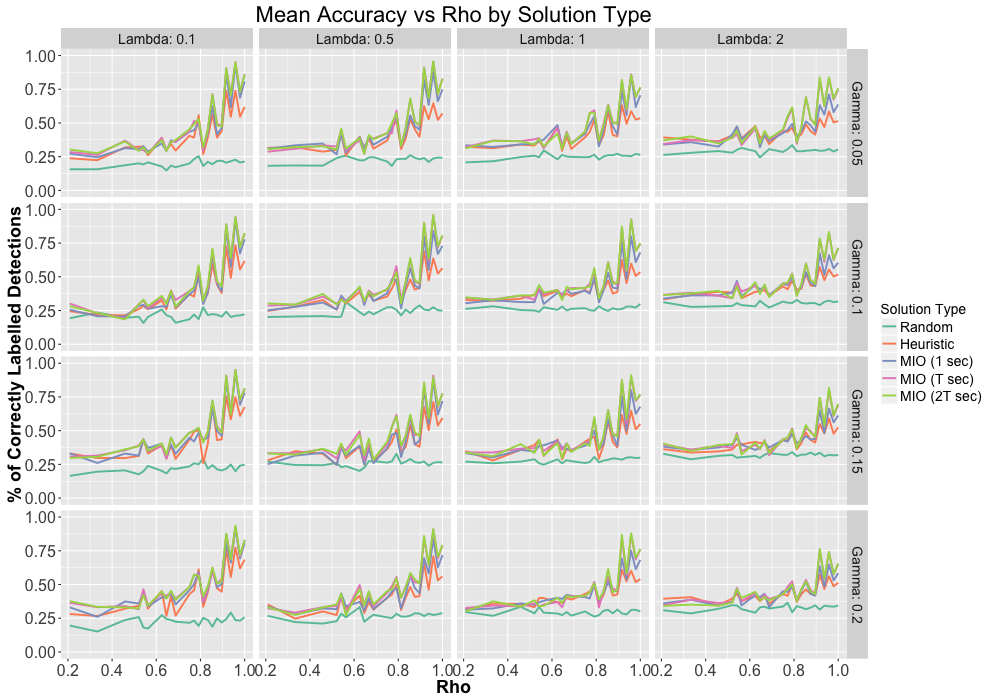
\includegraphics[width=\columnwidth]{../Figures/4_8_Accuracy}
  \caption{Accuracy of robust heuristic and MIO as compared to random solutions for scenarios of 4 targets and 8 scans, arranged by $\gamma$ and $\lambda$.}
  \label{fig:Robust_4_8_Accuracy}
\end{figure}

\begin{figure}[ht]
  \centering
  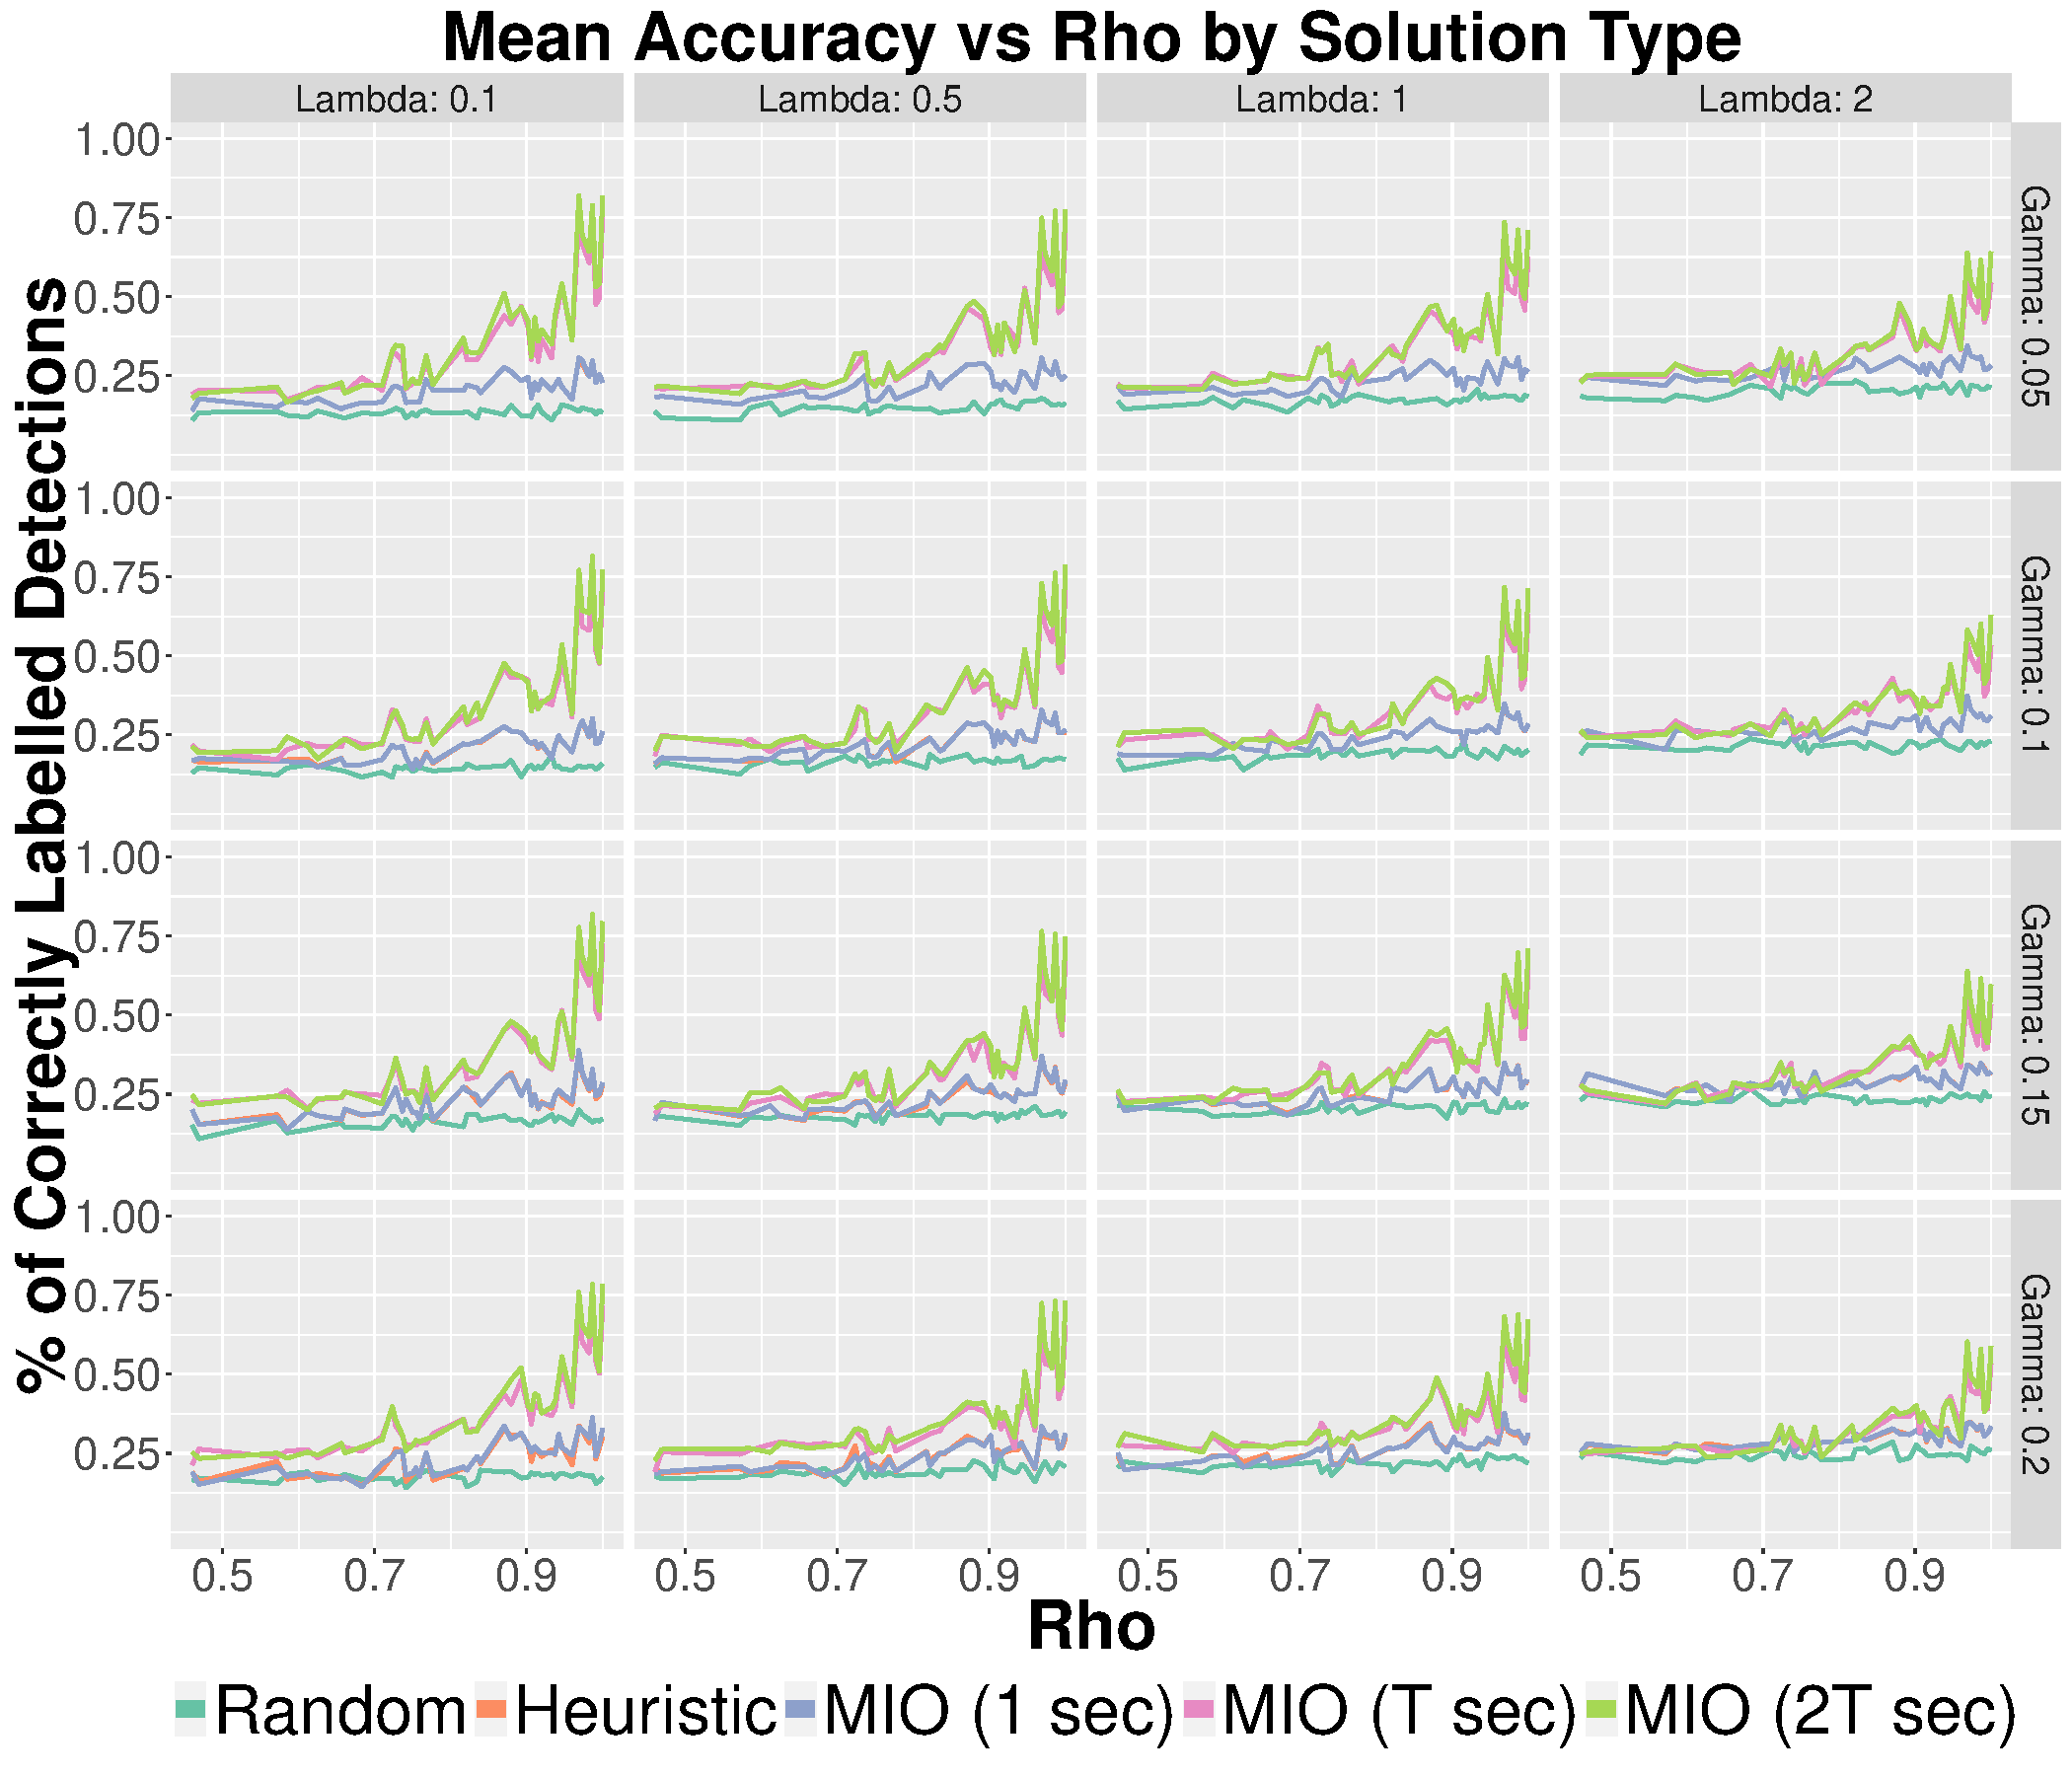
\includegraphics[width=\columnwidth]{../Figures/8_8_Accuracy}
  \caption{Accuracy of robust heuristic and MIO as compared to random solutions for scenarios of 8 targets and 8 scans, arranged by $\gamma$ and $\lambda$.}
  \label{fig:Robust_8_8_Accuracy}
\end{figure}

Similar to the performance of the basic heuristic, we again see that the robust heuristic improves greatly over that of a random solution, and the MIO offers even further improvement. Again, we seeing that running the MIO for 1 second offers significant improvements over the heuristic, and running the MIO for T seconds offers further improvement. However, running the MIO for 2T seconds offers little to no further improvement. Again, these results support the use of the MIO in an online algorithm with a sliding window as mentioned previously. 

Comparing Figure~\ref{fig:Robust_4_8_Accuracy} with the 4 target and 8 scan element of Figure~\ref{fig:Basic_Accuracy_Summary}, we see only a slight decrease in performance when $\gamma = 0.05$ and $\lambda=0.1$. This is an important result because we no longer know the number of targets in the robust case, yet we achieve almost the same levels of accuracy. Furthermore, both Figure~\ref{fig:Robust_4_8_Accuracy} and Figure~\ref{fig:Robust_8_8_Accuracy} show that the robust algorithms are more robust to decreases in the detection probability $\gamma$ than to increases in the false alarm rate $\lambda$. We conclude that the robust approaches are more sensitive to changes in the false alarm rate, in particular when it comes to making data associations. 

We have shown that both the heuristic and the MIO tend to underestimate the number of targets, due to the chosen penalties. We have also shown that accuracy degrades as the false alarm rate increases. This is likely not a coincidence. It is probable that as a result of underestimation, in which fewer trajectories are generated, there is a higher rate of misclassification of detections as false alarms, which in turn directly leads to a reduced accuracy. Therefore, it is a promising result to see accuracies above 75\% in Figure~\ref{fig:Robust_8_8_Accuracy}, even when Figure~\ref{fig:Robust_8_8_Histogram} suggests overestimation. It is entirely possible that further parameter tuning or introducing more complex penalties would lead to even great performance in the data association problem.

\subsubsection{Trajectory Estimation}
We conclude our analysis of the robust approaches with a discussion on their performance in the sphere of the trajectory estimation problem. Figures~\ref{fig:Robust_4_8_Delta} and~\ref{fig:Robust_8_8_Delta} plot the $\delta$ performance metric against the difficulty metric, $\sigma$, for scenarios of four and eight targets, respectively. Again, both scenarios have eight scans and both Figures have been arranged by $\gamma$ and $\lambda$. Note that the range on $\sigma$ has been reduced from $[0.1,5.0]$ to $[0.1, 2.0]$. 

\begin{figure}[ht]
  \centering
  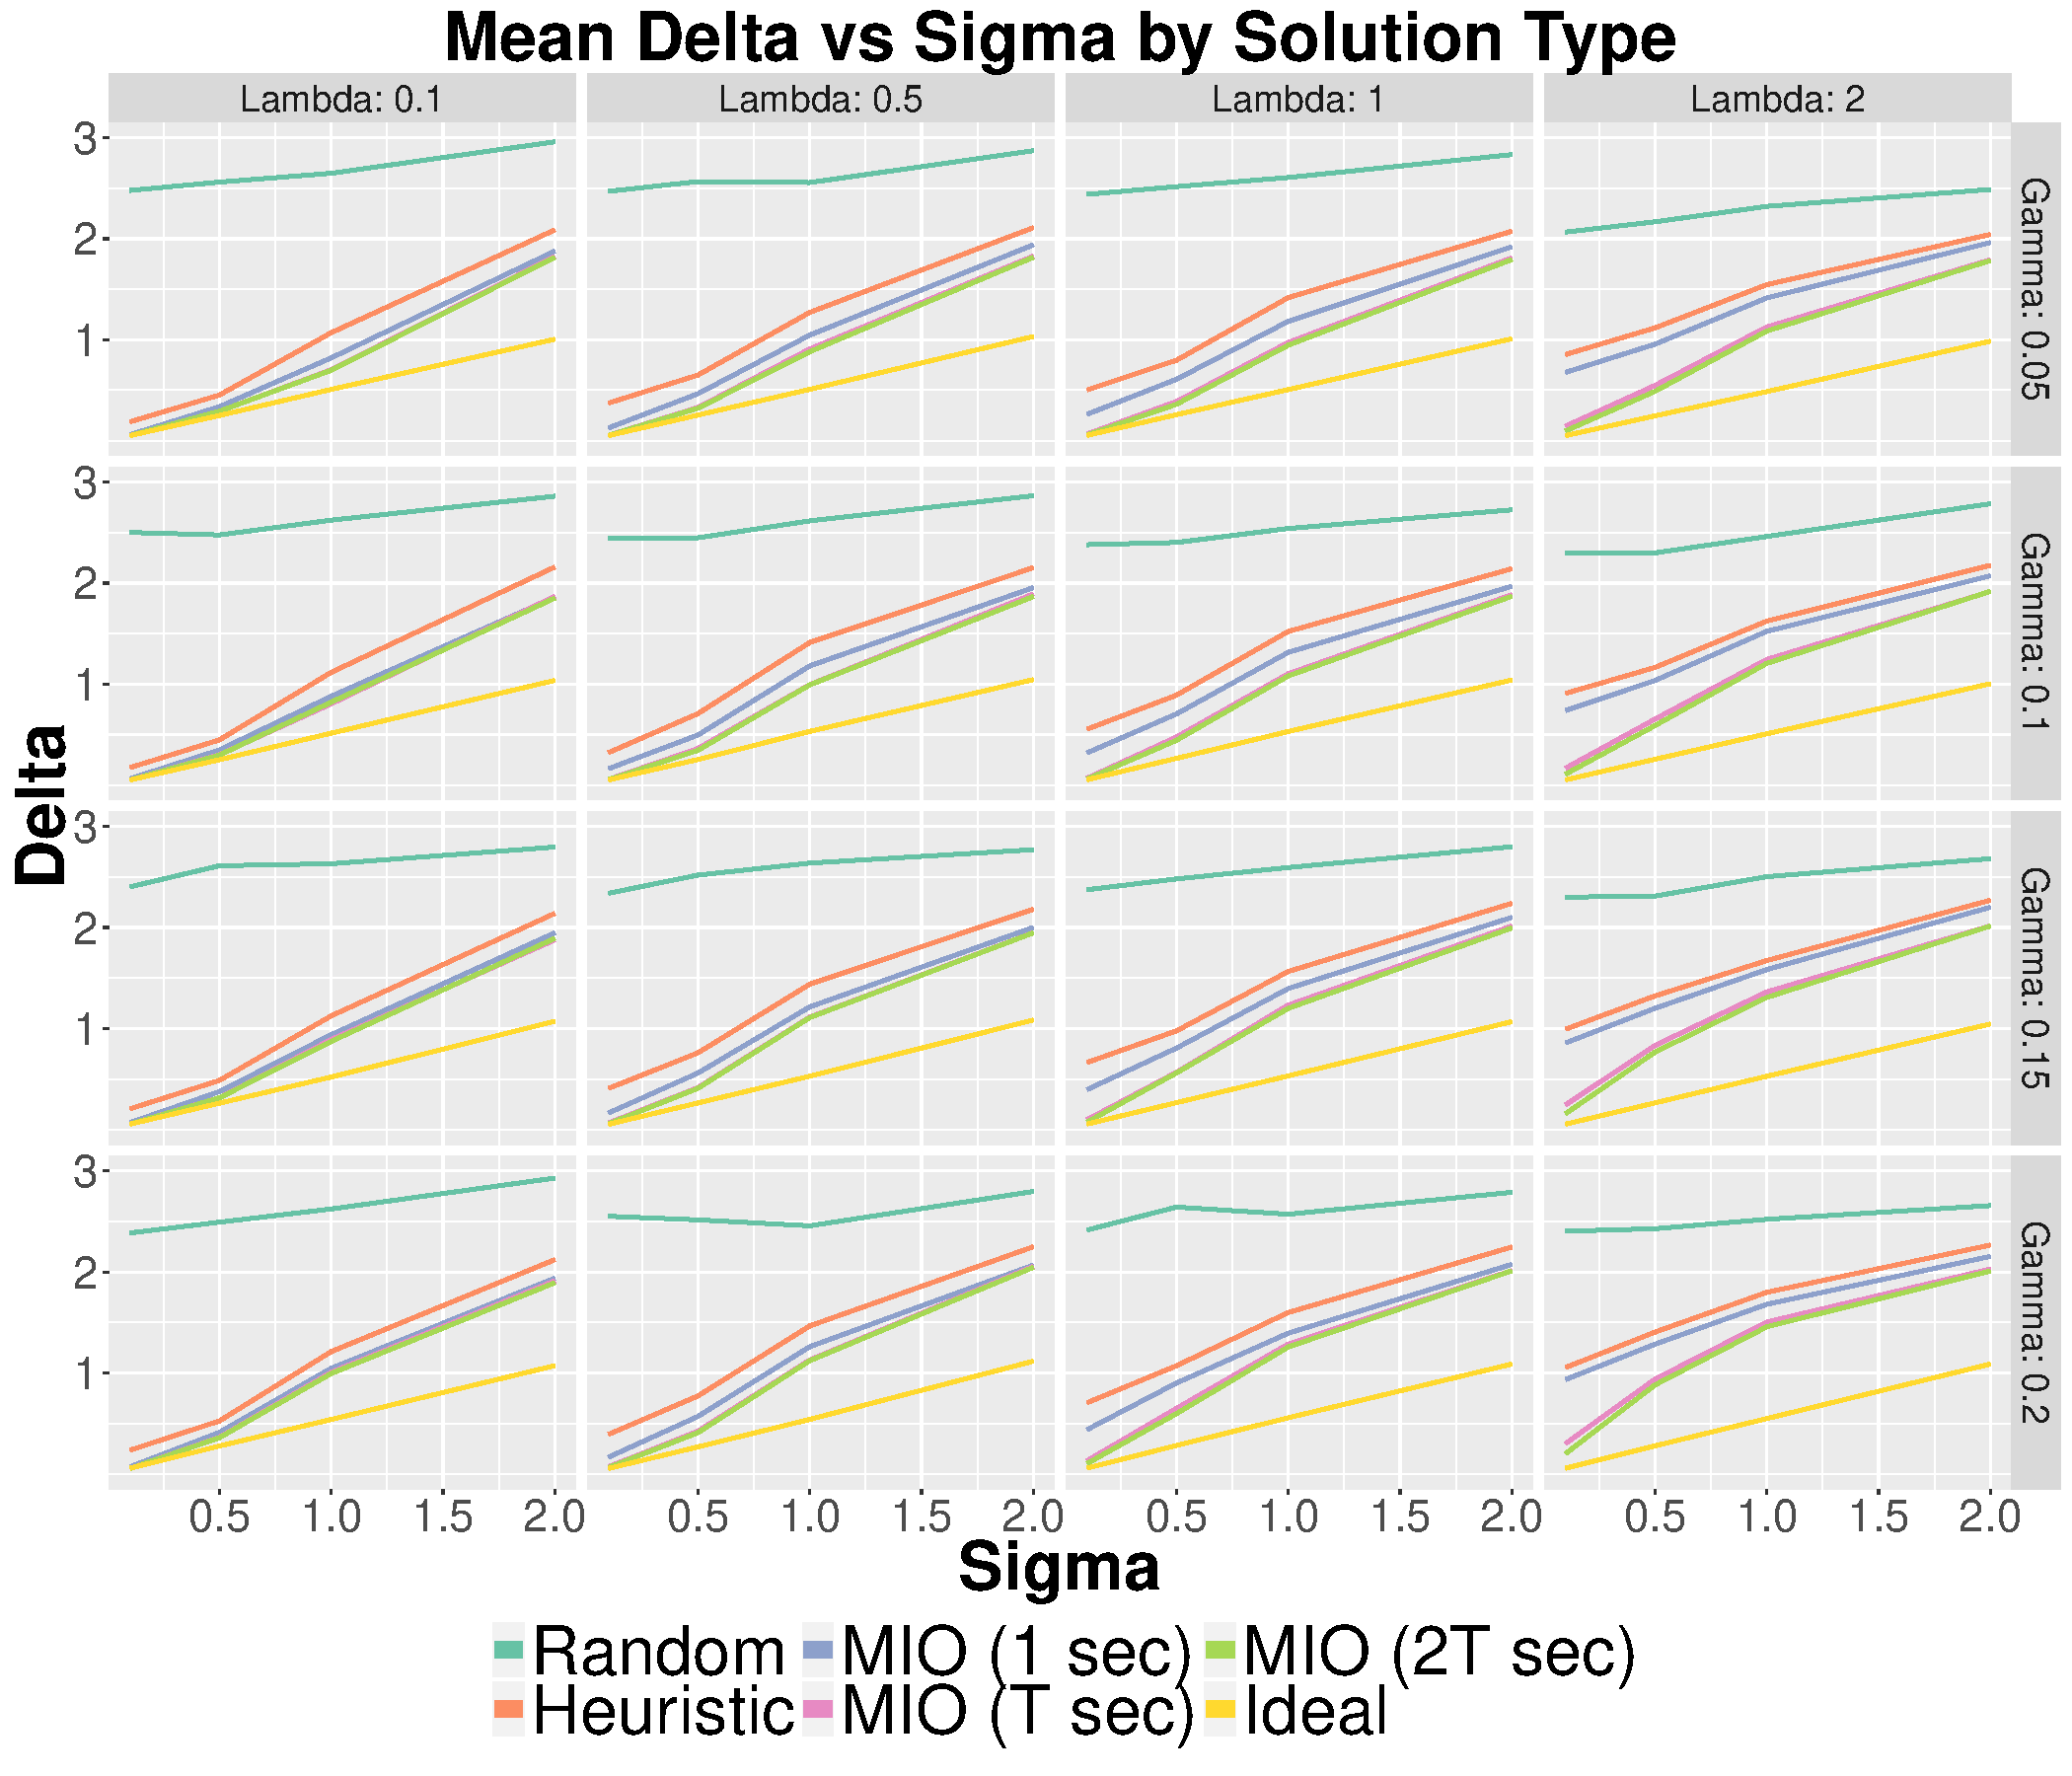
\includegraphics[width=\columnwidth]{../Figures/4_8_Delta}
  \caption{$\delta$ of robust heuristic and MIO as compared to random solutions for scenarios of 4 targets and 8 scans.}
  \label{fig:Robust_4_8_Delta}
\end{figure}

\begin{figure}[ht]
  \centering
  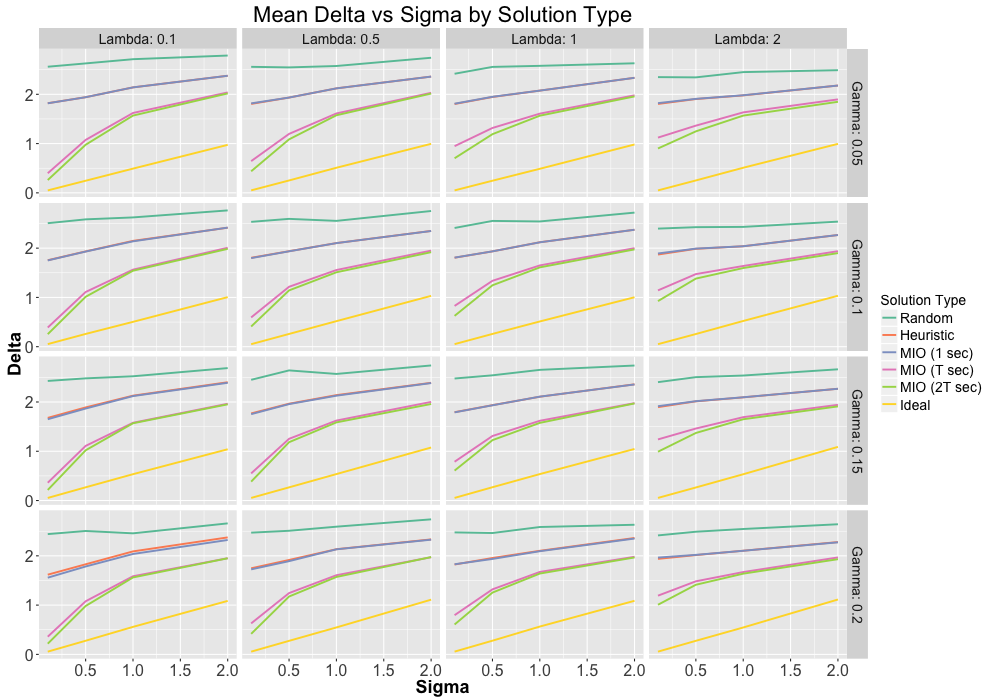
\includegraphics[width=\columnwidth]{../Figures/8_8_Delta}
  \caption{$\delta$ of robust heuristic and MIO as compared to random solutions for scenarios of 8 targets and 8 scans.}
  \label{fig:Robust_8_8_Delta}
\end{figure}

Again, we measure against the basic approaches by comparing Figure~\ref{fig:Robust_4_8_Delta} with the 4 target and 8 scan element of Figure~\ref{Fig:Basic_Delta_Summary}. We see that the robust approaches do not drastically reduce in performance for the easiest robust scenario of $\gamma = 0.05$ and $\lambda = 0.1$. However, the gap in performance between the ideal solution and the solutions of the robust algorithms grows wider with increases in $\sigma$, something that is expected but was not as sizable in the basic experiment. Therefore, the robust approaches may be less robust to increases in $\sigma$ in scenarios with detection ambiguity. However, it also appears that these methods are more robust to increases in the false alarm rate $\lambda$ when it comes to trajectory estimation than they were when it came to data association, especially in the larger scenario shown in Figure~\ref{fig:Robust_8_8_Delta}. We conclude that our robust methods are fairly robust to both increases in the false alarm rate and decreases in trajectory estimation under detection ambiguity, but increasing the signal noise degrades the performance of our methods more so in scenarios with detection ambiguity than in scenarios without detection ambiguity.

In summary,.....discussion on robust summary


